
%%%%%%%%%%%%%%%%%%%%%%%%%%%%%%%%%%%%%%%%%%%%%%%%%%%%
% Document type, global settings, and packages
%%%%%%%%%%%%%%%%%%%%%%%%%%%%%%%%%%%%%%%%%%%%%%%%%%%%

\documentclass[12pt,amsmath]{report}   %12 point font for Times New Roman
\usepackage{graphicx}  %for images and plots
\usepackage[letterpaper, left=1.5in, right=1in, top=1in, bottom=1in]{geometry}
\usepackage{setspace}  %use this package to set linespacing as desired
\usepackage{times}  %set Times New Roman as the font
\usepackage[explicit]{titlesec}  %title control and formatting
\usepackage[titles]{tocloft}  %table of contents control and formatting
\usepackage[backend=bibtex, sorting=none, bibstyle=ieee]{biblatex}  %reference manager
\usepackage[bookmarks=true, hidelinks]{hyperref}
\usepackage[page]{appendix}  %for appendices
\usepackage{rotating}  %for rotated, landscape images

\usepackage[normalem]{ulem}  %for italicized text
\usepackage{amssymb}
\usepackage{amsmath}
\usepackage{bm}
\usepackage{mathtools}

%\newenvironment{psmallmatrix}
 % {\left(\begin{smallmatrix}}
  % {\end{smallmatrix}\right)}

%%%%%%%%%%%%%%%%%%%%%%%%%%%%%%%%%%%
% Bibliography
%%%%%%%%%%%%%%%%%%%%%%%%%%%%%%%%%%%

%Add your bibliography file here
\bibliography{references}

% prevent certain fields in references from printing in bibliography
\AtEveryBibitem{\clearfield{issn}}
\AtEveryBibitem{\clearlist{issn}}

\AtEveryBibitem{\clearfield{language}}
\AtEveryBibitem{\clearlist{language}}

\AtEveryBibitem{\clearfield{doi}}
\AtEveryBibitem{\clearlist{doi}}

\AtEveryBibitem{\clearfield{url}}
\AtEveryBibitem{\clearlist{url}}

\AtEveryBibitem{%



  
      \ifentrytype{online}
    {}
    
    {\clearfield{urlyear}\clearfield{urlmonth}\clearfield{urlday}}}

%%%%%%%%%%%%%%%%%%%%%%
% Start of Document
%%%%%%%%%%%%%%%%%%%%%%

\begin{document}
\doublespacing  %set line spacing

%%%%%%%%%%%%%%%%%%%%%%%%%%%%%%%%%%%%%
% Title Page
%%%%%%%%%%%%%%%%%%%%%%%%%%%%%%%%%%%%%

%% Define your thesis title, your name, your school, and your month and year of graduation here

\newcommand{\thesisTitle}{Quantum State Control of Trapped Ions for Computation and Multi-Ensemble Atomic Clocks}
\newcommand{\yourName}{Thomas E. deLaubenfels}
\newcommand{\yourSchool}{Physics}
\newcommand{\yourMonth}{December}
\newcommand{\yourYear}{2017}

%%%%%%%%%%%%%%%%%%%%%%%%%%%%%%%%%%%%%%%%%%%%%%%%%%%%%%%%%
% Do not edit these lines unless you wish to customize
% the template
%%%%%%%%%%%%%%%%%%%%%%%%%%%%%%%%%%%%%%%%%%%%%%%%%%%%%%%%%



\begin{titlepage}
\begin{center}

\begin{singlespacing}

\textbf{\MakeUppercase{\thesisTitle}}\\
\vspace{10\baselineskip}
A Dissertation\\
Presented to\\
The Academic Faculty\\
\vspace{3\baselineskip}
By\\
\vspace{3\baselineskip}
\yourName\\
\vspace{3\baselineskip}
In Partial Fulfillment\\
of the Requirements for the Degree\\
Doctor of Philosophy in the\\
School of \yourSchool\\
\vspace{3\baselineskip}
Georgia Institute of Technology\\
\vspace{\baselineskip}
\yourMonth{} \yourYear{}
\vfill
Copyright \copyright{} \yourName{} \yourYear{}

\end{singlespacing}

\end{center}
\end{titlepage}



\currentpdfbookmark{Title Page}{titlePage}  %add PDF bookmark for this page

%%%%%%%%%%%%%%%%%%%%%%%%%%%%%%%%%%%%%
% Approval Page
%%%%%%%%%%%%%%%%%%%%%%%%%%%%%%%%%%%%%

%% Define your committee members. If you have less than 6, simple delete/comment the unused lines

\newcommand{\committeeMemberOne}{Dr. Kenneth Brown, Advisor}
\newcommand{\committeeMemberOneDepartment}{School of Chemistry \& Biochemistry and School of Physics}
\newcommand{\committeeMemberOneAffiliation}{Georgia Institute of Technology}

\newcommand{\committeeMemberTwo}{Dr. Brian Kennedy}
\newcommand{\committeeMemberTwoDepartment}{School of Physics}
\newcommand{\committeeMemberTwoAffiliation}{Georgia Institute of Technology}

\newcommand{\committeeMemberThree}{Dr. Michael Chapman}
\newcommand{\committeeMemberThreeDepartment}{School of Physics}
\newcommand{\committeeMemberThreeAffiliation}{Georgia Institute of Technology}

\newcommand{\committeeMemberFour}{Dr. Facundo Fernandez}
\newcommand{\committeeMemberFourDepartment}{School of Chemistry \& Biochemistry}
\newcommand{\committeeMemberFourAffiliation}{Georgia Institute of Technology}

\newcommand{\committeeMemberFive}{Dr. Colin Parker}
\newcommand{\committeeMemberFiveDepartment}{School of Physics}
\newcommand{\committeeMemberFiveAffiliation}{Georgia Institute of Technology}

\newcommand{\approvalDay}{14}
\newcommand{\approvalMonth}{July}
\newcommand{\approvalYear}{2017}

%%%%%%%%%%%%%%%%%%%%%%%%%%%%%%%%%%%%%%%%%%%%%%%%%%%%%%%%%
% Do not edit these lines unless you wish to customize
% the template
%%%%%%%%%%%%%%%%%%%%%%%%%%%%%%%%%%%%%%%%%%%%%%%%%%%%%%%%%


\begin{titlepage}
\begin{singlespacing}
\begin{center}

\textbf{\MakeUppercase{\thesisTitle}}\\
\vspace{10\baselineskip}

\end{center}
\vfill

%Define minipages, depending on how many authors there are
\ifdefined\committeeMemberFour

Approved by:
\vspace{2\baselineskip}		%adjust the number in front of "\baselineskip" for alignment

\begin{minipage}[b]{0.4\textwidth}
	
	\committeeMemberOne\\
	\committeeMemberOneDepartment\\
	\textit{\committeeMemberOneAffiliation}\\
	
	\committeeMemberTwo\\
	\committeeMemberTwoDepartment\\
	\textit{\committeeMemberTwoAffiliation}\\
	
	\committeeMemberThree\\
	\committeeMemberThreeDepartment\\
	\textit{\committeeMemberThreeAffiliation}\\
	
	\vspace{2\baselineskip}		%adjust the number in front of "\baselineskip" for alignment
	
\end{minipage}
\hspace{0.1\textwidth}
\begin{minipage}[b]{0.4\textwidth}
	
	\committeeMemberFour\\
	\committeeMemberFourDepartment\\
	\textit{\committeeMemberFourAffiliation}\\
	
	\ifdefined\committeeMemberSix
	\committeeMemberFive\\
	\committeeMemberFiveDepartment\\
	\textit{\committeeMemberFiveAffiliation}\\
	
	\committeeMemberSix\\
	\committeeMemberSixDepartment\\
	\textit{\committeeMemberSixAffiliation}\\
	
	Date Approved: \approvalMonth{} \approvalDay, \approvalYear
	\vspace{1\baselineskip}		%adjust the number in front of "\baselineskip" for alignment
	
	\else
	
	\committeeMemberFive\\
	\committeeMemberFiveDepartment\\
	\textit{\committeeMemberFiveAffiliation}\\
		
	Date Approved: \approvalMonth{} \approvalDay, \approvalYear
	\vspace{5\baselineskip}		%adjust the number in front of "\baselineskip" for alignment
	
	\fi
	
\end{minipage}

\else

\hspace{0.6\textwidth}
\begin{minipage}[b]{0.4\textwidth}
	
	Approved by:
	\vspace{2\baselineskip}		%adjust the number in front of "\baselineskip" for alignment
	
	\committeeMemberOne\\
	\committeeMemberOneDepartment\\
	\textit{\committeeMemberOneAffiliation}\\
	
	\committeeMemberTwo\\
	\committeeMemberTwoDepartment\\
	\textit{\committeeMemberTwoAffiliation}\\
	
	\committeeMemberThree\\
	\committeeMemberThreeDepartment\\
	\textit{\committeeMemberThreeAffiliation}\\
	
	\vspace{2\baselineskip}		%adjust the number in front of "\baselineskip" for alignment
	
	Date Approved: \approvalMonth{} \approvalDay, \approvalYear
	\vspace{\baselineskip}		%adjust the number in front of "\baselineskip" for alignment
	
\end{minipage}

\fi





\end{singlespacing}
\end{titlepage}


%%%%%%%%%%%%%%%%%%%%%%%%%%%%%%%%%%%%%
% Epigraph
%%%%%%%%%%%%%%%%%%%%%%%%%%%%%%%%%%%%%

%% Define your quote and author for the epigraph here

\newcommand{\yourQuote}{''They don't think it be like it is, but it do.''}
\newcommand{\yourAuthor}{Jazzy}

%%%%%%%%%%%%%%%%%%%%%%%%%%%%%%%%%%%%%%%%%%%%%%%%%%%%%%%%%
% Do not edit these lines unless you wish to customize
% the template
%%%%%%%%%%%%%%%%%%%%%%%%%%%%%%%%%%%%%%%%%%%%%%%%%%%%%%%%%

\begin{titlepage}
\begin{center}

\vspace*{\fill}
\yourQuote\\
\textit{\yourAuthor}
\vspace*{\fill}

\end{center}
\end{titlepage}



%%%%%%%%%%%%%%%%%%%%%%%%%%%%%%%%%%%%%
% Dedication
%%%%%%%%%%%%%%%%%%%%%%%%%%%%%%%%%%%%%

%% Define your dedication statement here

\newcommand{\yourDedication}{For Allie and Jazzy.}

%%%%%%%%%%%%%%%%%%%%%%%%%%%%%%%%%%%%%%%%%%%%%%%%%%%%%%%%%
% Do not edit these lines unless you wish to customize
% the template
%%%%%%%%%%%%%%%%%%%%%%%%%%%%%%%%%%%%%%%%%%%%%%%%%%%%%%%%%

\begin{titlepage}
\begin{center}

\vspace*{\fill}
\yourDedication\\
\vspace*{\fill}

\end{center}
\end{titlepage}


%%%%%%%%%%%%%%%%%%%%%%%%%%%%%%%%%%%%%
% Acknowledgments
%%%%%%%%%%%%%%%%%%%%%%%%%%%%%%%%%%%%%

\pagenumbering{roman}
\addcontentsline{toc}{chapter}{Acknowledgments}
\setcounter{page}{3} % set the page number appropriately based on the number of intro pages


\clearpage
\begin{centering}
\textbf{ACKNOWLEDGEMENTS}\\
\vspace{\baselineskip}
\end{centering}

I owe substantial thanks and gratitude to my two thesis advisors, Jason Amini and Ken Brown, without whom I would never have seen the far side of my doctorate. Much more could be said of their support, patience, and imparted knowledge than would reasonably fit here in the preamble, but suffice to say I couldn't have asked for better mentors. Many thanks as well to Bob Wyllie, who took on a similar role during my final year. 

I am indebted to the whole of the Quantum Systems lab at GTRI for giving me the opportunity and resources to conduct all of the research presented here. It was a pleasure to have been part of the lab for the last 4 years. I'd like to especially thank Bob Wylie, Brian Sawyer, Brian McMahon, True Merrill, and Wade Rellergert for their ongoing help and dissemination of knowledge. 

Finally, I would like to thank Elena for all of her love and support throughout this final leg. 



\clearpage
%\pagenumbering{gobble}  %remove page number on summary page


%\addtocontents{toc}{\cftpagenumbersoff{chapter}} 

%\currentpdfbookmark{Acknowledgments}{acknowledgments}
%\addtocontents{toc}{\cftpagenumberson{chapter}} 

%%%%%%%%%%%%%%%%%%%%%%%%%%%%%%%%%%%%%
% Table of Contents
%%%%%%%%%%%%%%%%%%%%%%%%%%%%%%%%%%%%%

% Format for Table of Contents
\renewcommand{\cftchapdotsep}{\cftdotsep}  %add dot separators

\renewcommand{\cftchapfont}{\bfseries}  %set title font weight
\renewcommand{\cftchappagefont}{}  %set page number font weight
\renewcommand{\cftchappresnum}{Chapter }
\renewcommand{\cftchapaftersnum}{:}
\renewcommand{\cftchapnumwidth}{5em}
\renewcommand{\cftchapafterpnum}{\vskip\baselineskip} %set correct spacing for entries in single space environment
\renewcommand{\cftsecafterpnum}{\vskip\baselineskip}  %set correct spacing for entries in single space environment
\renewcommand{\cftsubsecafterpnum}{\vskip\baselineskip} %set correct spacing for entries in single space environment
\renewcommand{\cftsubsubsecafterpnum}{\vskip\baselineskip} %set correct spacing for entries in single space environment

%format title font size and position (this also applys to list of figures and list of tables)
\titleformat{\chapter}[display]
{\normalfont\bfseries\filcenter}{\chaptertitlename\ \thechapter}{0pt}{\MakeUppercase{#1}}

\renewcommand\contentsname{Table of Contents}

\begin{singlespace}
\tableofcontents
\end{singlespace}

\currentpdfbookmark{Table of Contents}{TOC}

\clearpage

%%%%%%%%%%%%%%%%%%%%%%%%%%%%%%%%%%%%%
% List of figures and tables
%%%%%%%%%%%%%%%%%%%%%%%%%%%%%%%%%%%%%

\addcontentsline{toc}{chapter}{List of Tables}
\begin{singlespace}
	\setlength\cftbeforetabskip{\baselineskip}  %manually set spacing between entries
	\listoftables
\end{singlespace}

\clearpage

\addcontentsline{toc}{chapter}{List of Figures}
\begin{singlespace}
\setlength\cftbeforefigskip{\baselineskip}  %manually set spacing between entries
\listoffigures
\end{singlespace}

\clearpage

%%%%%%%%%%%%%%%%%%%%%%%%%%%%%%%%%%%%%%%%%%%%%%%%%%%%%%%%%%%%%%%%%
% This is the Summary (abstract should be separate document)
%%%%%%%%%%%%%%%%%%%%%%%%%%%%%%%%%%%%%%%%%%%%%%%%%%%%%%%%%%%%%%%%%

\clearpage
\begin{centering}
\textbf{SUMMARY}\\
\vspace{\baselineskip}
\end{centering}



%\pagenumbering{gobble}  %remove page number on summary page

The purpose of this work is to investigate methods by which the quantum states of trapped ions may be better controlled and measured for the applications of quantum computing, quantum simulation, and the generation of atomic frequency standards. We report on two primary projects: first, we control the relative coupling strengths of carrier and first-order motional sideband interactions of a trapped ion by placing it in a resonant optical standing wave. Our configuration uses the surface of a microfabricated chip trap as a mirror, avoiding the technical challenges of in-vacuum optical cavities. Displacing the ion along the standing wave, we show a periodic suppression of the carrier and sideband transitions, with the cycles for the two cases 180$^{\circ}$ out of phase with each other. This technique allows for the suppression of off-resonant carrier excitations when addressing the motional sidebands, and has applications in quantum computation and quantum simulation. Second, we investigate methods proposed in Ref. \cite{BorregaardSorensen} which may improve the performance of trapped ion (or atom) frequency standards when the interrogating local oscillator is of limited quality. These methods could be applied to future generations of small-scale frequency standards, which are in demand for applications such as local GPS networks and distributed sensors. We propose a scheme for  implementing these methods in a $^{40}$Ca$^+$ based frequency standard, and outline the technical requirements for doing so. Finally, we present preliminary results characterizing single-ion coherence times and ion ``state destruction'' events in our system, and discuss how they will affect the realization of the proposed scheme. 

%%%%%%%%%%%%%%%%%%%%%%%%%%%%
%
% Chapters
%
%%%%%%%%%%%%%%%%%%%%%%%%%%%%

%%%%%%%%%%%%%%%%%%%%%%
% formatting
%%%%%%%%%%%%%%%%%%%%%%

% resume page numbering for rest of document

\pagenumbering{arabic}
\setcounter{page}{1} % set the page number appropriately

% Adjust chapter title formatting
\titleformat{\chapter}[display]
{\normalfont\bfseries\filcenter}{\MakeUppercase\chaptertitlename\ \thechapter}{0pt}{\MakeUppercase{#1}}  %spacing between titles
\titlespacing*{\chapter}
  {0pt}{0pt}{30pt}	%controls vertical margins on title
  
% Adjust section title formatting
\titleformat{\section}{\normalfont\bfseries}{\thesection}{1em}{#1}

% Adjust subsection title formatting
\titleformat{\subsection}{\normalfont}{\uline{\thesubsection}}{0em}{\uline{\hspace{1em}#1}}

% Adjust subsubsection title formatting
\titleformat{\subsubsection}{\normalfont\itshape}{\thesubsection}{1em}{#1}

%%%%%%%%%%%%%%%%
% Chapter 1
%%%%%%%%%%%%%%%%

\chapter{Introduction and Background}

Within the last several decades it has become possible to control and measure the state of various quantum systems with an increasing level of sophistication \cite{doi:10.1080/09500349708231863, QuantMeas}. In addition to providing the experimental basis to test fundamental aspects of quantum theory \cite{QuantTh}, practical applications of these techniques have given rise to the concept of ``quantum technology'' for uses such as sensing, metrology, microscopy, computation, simulation, information processing, cryptography, electronics and photonics, frequency standard generation, etc \cite{QuantMeas, Dowling1655}. Trapped ion systems are one choice of system that can realize many of these applications. Although they are well researched and offer a good degree of state control and measurement, there remain a variety of technical challenges and limitations which must be accounted for when using trapped ions as a platform for such technologies. The purpose of this work is to investigate methods by which the quantum state of trapped ions may be better controlled and measured for the particular applications of quantum computing, quantum simulation, and the generation of atomic frequency standards.

\section{On motional state control for computation and simulation}

The design of electromagnetic ion traps such as Penning or Paul traps leads to confining potentials that are effectively harmonic. As we'll see in the technical review provided in Ch. 2, the internal electronic states of trapped ions become coupled with the motional states when the ions interact with resonant light fields. This allows the motional states to be coherently controlled, leading to a variety of important applications. For instance, the coupling takes the form of an almost ideal Jaynes-Cummings interaction \cite{Jaynes63.IEEE.51.89}, allowing trapped ion systems to function as a platform for a variety of cavity QED experiments \cite{CavityQED,Wu97.PRL.78.3086}, as well as enabling the analysis of various non-classical motional states (such as Fock and squeezed states) \cite{PhysRevA.49.1202,PhysRevLett.76.1796}. As another example, the ability to coherently control the motional states forms the basis for two-qubit gates in ion trap quantum computation \cite{Cirac95.PRL.74.4091,Sorensen00.PRA.62.022311,Schmidt03.Nature.422.408}. 

Control of the motional states is often achieved by interacting with the ion on its motional sidebands. These interactions are also used for cooling ions to the motional ground state \cite{Diedrich89.PRL.62.403}, measuring ion heating rates \cite{Turchette.PRA.61.063418,Shu14.PRA.89.062308}, and identifying and cooling molecular ions \cite{Goeders13.JPhysChemA.117.9725,Rugango15.NJP.17.035009,Wan15.PRA.91.043425}. The speed at which these interactions can take place depends on the intensity of the exciting radiation. Due to spectral broadening, off-resonant coupling to the primary transition (evident either as motion independent population transfer or an AC Stark shift), places a limit on the speed of the sideband interactions. Suppressing the primary transition, referred to also as the carrier, can remove this limit and, in particular, would allow for improved two-qubit gate fidelities as the gate time becomes comparable or shorter than a cycle of the harmonic motion \cite{Sorensen00.PRA.62.022311,Mizrahi14.APB.114.45}. Suppression of the carrier also has applications in quantum simulation.  For instance, trapped ions have been proposed as a system for modeling the expansion of the universe \cite{Menicucci10.NJP.12.095019}. The simulation requires off-resonant excitation of both the red and blue sidebands by a red-detuned exciting field, with no coupling to the carrier. Because the blue sideband is both weaker and further from resonance than the carrier transition, suppression of the carrier is important for such an experiment. 

Replacing running wave optical beams with standing wave beams provides a method to selectively suppress the carrier and reduce off-resonant excitations when addressing the motional sidebands \cite{Cirac92.PRA.46.2668,Zhang12.PRA.85.053420}. In such a configuration, the coupling strengths of the carrier and sidebands acquire a periodic dependence on the atom's spatial position within the standing wave fringes \cite{Cirac92.PRA.46.2668,James98.APB.66.181}, with the cycles for the two cases $180^\circ$ out of phase with each other. This periodic dependence of the coupling strengths has been demonstrated in cavity experiments with trapped ions \cite{Leibrandt09.PRL.103.103001,Guthohrlein01.Nature.414.49,Steiner13.PRL.110.043003,PhysRevLett.89.103001}. However, the use of cavities involves technical challenges such as the alignment of optics in vacuum and the tendency for optics and dielectric mirrors to become charged, complicating the integration of cavities with microfabricated ion traps \cite{Harlander10.NJP.9.093035,Clark14.PRAppl.1.024004}.

In Ch. 4 of this work we demonstrate the same position dependence in a standing wave field produced by a single mirror, which in this case is simply the surface of a planar ion trap. This configuration has the advantage of being simpler to implement than an optical cavity. In order to account for imperfect beam alignment, reflection losses, and similar system limitations, we extend the calculations of Refs.~\cite{Cirac92.PRA.46.2668,James98.APB.66.181} to the case of non-normal incidence laser beams and unequal couplings of the incident and reflected laser beams with the ion. In doing so, we find a criterion for the out of phase carrier and sideband coupling strengths that is set by the incident angle of the laser beam and the orientation of the ion's harmonic motion. Furthermore, by using the position dependence of the coupling strengths within the standing wave fringes, we are able measure the ion's relative position as a function of applied electric field in order to map the trapping potentials. These results are compared with those given by numerical models of the trap system.

\section{On the improvement of atomic frequency standards}

Atomic frequency standards (colloquially called atomic clocks) are the most accurate time and frequency standards known, and serve as references for GPS satellites, sensors, television broadcasts, and any other applications which require precision time keeping. These devices use radiation from a local oscillator (LO) to excite atomic transitions, allowing the LO to be stabilized to the transition resonance. The first such device to be built was completed in 1949 and was based on an ammonia absorption line at 24 GHz. Although it was successful as a proof-of-concept, its performance (measured by fractional frequency offsets $\Delta f / f_0$ of $10^{-7} - 10^{-8}$) could not match the best quartz standards at the time (with offsets around $2 \times 10^{-8}$) \cite{nistclocks, ammoniaclock}. By the mid 1950s, however, cesium beam standards based on the 9.2 GHz hyperfine transition were demonstrating fractional offsets of approximately $10^{-9}$ \cite{firstCs}, overtaking quartz oscillators. This marked the beginning of the atomic timekeeping era. Modern cesium standards used to define the SI second have fractional offsets on the order of $10^{-16}$ \cite{nistf2}, whereas frequency standards based on optical transitions (i.e. reference frequencies in the $10^{14}$ Hz range) have achieved stabilities of $\sigma_y (\tau) \sim 10^{-17} / \sqrt{\tau}$ \cite{OpticalClocks} ($\sigma_y$ being the Allan variance, which will be discussed in Ch. 5). Regardless of the choice in reference frequency,  devices on the bleeding edge of accuracy are limited to laboratory use due to their size and sensitivity to environmental factors such as vibration and temperature. These fixed-position standards are sufficient so long as the reference signal can be distributed beyond the lab. Currently this is done via global GPS signals, but the fragile nature of the GPS signal is a functional concern, particularly to the US armed forces. There is a recognized need to miniaturize these frequency standard technologies and make them sufficiently robust for field use in order to synchronize local GPS networks and distributed sensors. This demand for frequency references with reduced size, weight, and operating power has previously manifested in programs such as the DARPA IMPACT (BAA-08-32) and STOIC (BAA-14-41) programs. Most recently, the DARPA Atomic Clocks with Enhanced Stability (ACES) program (BAA-16-19) has sought an integrated clock in a package size of 50 cm$^3$ or less, with an operating power of 250 mW or less, and a stability $\sigma_y (\tau) < 10^{-11} / \sqrt{\tau}$ out to 10$^5$ s, matching the performance of a GPS locked reference or rack mount beam standard.

Trapped ion clocks are a good candidate for meeting such demands due to the demonstrated scalability of RF ion traps. For instance, in the QIS lab (where all of the work in this thesis was performed) we use planar chip traps on the order of 1 cm$^2$ that are designed in-house and fabricated at Georgia Tech using CMOS techniques (e.g. \cite{IonTrap}). However, the clock's performance depends both on the interrogation of the ions, which provides long term stability, and on the absence of noise in the LO, which provides the short term stability needed for interrogation. For references based on optical atomic transitions, the LO is a laser and is typically stabilized to an optical cavity. These cavities are generally heavy blocks of glass which provide rigidity against residual vibrational stress, and are otherwise isolated from environmental vibrations. Small package devices will require smaller, less stable cavities, resulting in much noisier LOs and diminished performance of the frequency reference. Microwave transitions can alternatively be used as reference frequencies, but such transitions (around $10^{10}$ Hz) are on the order of $10^4$ times less sensitive to fractional frequency shifts than optical transitions (around $10^{14}$ Hz). Maximizing the interrogation time of the atomic ensemble becomes critical in microwave based references in order to achieve maximum sensitivity. As in the optical case, the maximum interrogation time will be set by the LO performance. 

A proposal by Borregaard and S\o{}rensen \cite{BorregaardSorensen} describes how the performance of a trapped ion (or atom) clock may be improved when otherwise limited by a noisy LO. Specifically, their methods involve using multiple atomic ensembles in combination with adaptive measurement techniques in the trapped ion/atom clock in order to increase the interrogation time $T$ of the LO. This in turn  improves clock performance. In Ch. 5 of this work we investigate applying these methods to a $^{40}$Ca$^+$ based clock where the interrogating LO is a 729 nm laser (the same techniques will also be applicable to microwave based clocks). We consider the merits and technical requirements of such a system, and present a scheme of how it might be realized. Finally, with the goal of implementing this scheme, we report preliminary experimental data with regards to single-ion coherence times and state destruction during clock interrogations, and discuss how these technical barriers may be addressed.


%%%%%%%%%%%%%%%%
% Chapter 2
%%%%%%%%%%%%%%%%

\chapter{Ion trapping with {$^{40}$Ca$^+$}}

In this section we discuss the fundamental theory and principles of trapping and manipulating $^{40}$Ca$^+$ ions, which were used in all of the experiments described in this thesis. First we will discuss the fundamental principles of radio frequency (RF) traps which lead to approximately harmonic trapping potentials. We will then describe the characteristics and spectroscopy the of $^{40}$Ca$^+$ ion, the theory of laser-ion interactions, and other relevant experimental details that pertain to the state manipulation and measurement of this ion. 


%%%%%%%%%%%%%%%%%%%%%%%%%%%%%%%%%%%%%%%%%%%%%%%%%%%%%

\section{Radio frequency trap principles and ion dynamics}

A thorough review of ion trapping in radio frequency traps can be found in Refs. \cite{Wineland98.NIST.103.259, Leibfried03.RMP.75.281, Häffner2008155, Roos00.Thesis}. Here we will review the essential principles, as well as the resulting ion dynamics, that are relevant to our experiments. We assume that the ions will be trapped by a quadrupolar potential that can, near its center, be decomposed into static (DC) and sinusoidally varying (RF) components:
\begin{equation} 
\Phi (\textbf{r}, t) = \frac{U}{2} ( \alpha_x \ x^2 + \alpha_y \ y^2 + \alpha_z \ z^2 ) + \frac{V_{RF} \cos{(\Omega_{RF} t)}}{2} ( \alpha'_x \ x^2 + \alpha_y \ y^2 + \alpha_z \ z^2 ) \text{.}
\end{equation}
In our configuration we use an RF drive frequency $\approx$ 50 MHz. The geometric factors $\alpha_i$ and $\alpha'_i$ depend on the trap design and must satisfy the Laplace equation $\nabla^2 \Phi = 0$. In a linear trap configuration, the RF potential provides dynamic radial confinement in two radial dimensions while static potentials provide axial confinement in the third dimension. Choosing $z$ as our axial coordinate, we can use $\alpha_x + \alpha_y = - \alpha_z$, $\alpha'_x = - \alpha'_y$, and $\alpha'_z = 0$, which satisfies the Laplace equation. 

The classical equation of motion for a particle with charge $Q$ and mass $m$ is
\begin{equation}
\ddot{u} = - \frac{Q}{m} \frac{\partial \Phi}{\partial u} = - \frac{Q}{m} [ U \alpha_u + V_{RF}\cos{(\Omega_{RF} t)} \alpha'_u ] \ u
\end{equation}
and can be transformed into the canonical form of the Mathieu equation 
\begin{equation}
\frac{\partial^2 u}{\partial \xi^2} + [ a_u + 2 q_u \cos{(2 \xi)} ] \ u = 0 
\end{equation}
by the substitutions
\begin{equation}
\xi = \frac{1}{2} \Omega_{RF} \ t \text{,} \ \ \ \ \ \ \ \ a_u = \frac{4 Q U \alpha_u}{m \Omega_{RF}^2} \text{,} \ \ \ \ \ \ \ \ q_u = \frac{2 Q V_{RF} \ \alpha'_u}{m \Omega_{RF}^2} \ \text{.}
\end{equation}
Therefore, in the linear trap configuration the equations of motion near the center/null of the RF potential become
\begin{equation}
\begin{split}
\frac{\partial^2 x}{\partial \xi^2} + [ a_x + 2 q_x \cos{(2 \xi)} ] \ x = 0  \\
\frac{\partial^2 y}{\partial \xi^2} + [ a_y + 2 q_y \cos{(2 \xi)} ] \ y = 0  \\
\frac{\partial^2 x}{\partial \xi^2} +  a_z  \ z = 0 \ \text{.}
\end{split}
\end{equation}
The axial motion (in the $z$ direction) is harmonic and has frequency
\begin{equation}
\omega_z = \frac{\sqrt{a_z}}{2} \Omega_{RF} \text{.}
\end{equation}
The radial motion in the $xy$ plane is more complex and involves solutions to the Mathieu equation which contain recursive coefficients. In the limit of $|a_{x,y}|, q_{x,y}^2 \ll 1$, we can take the lowest order approximation of these solutions and obtain
\begin{equation}
\begin{split}
x(t) \propto \cos\big( \omega_x t \big) \big[1 - \frac{q_x}{2} \cos (\Omega_{RF} t) \big] \\
y(t) \propto \cos\big( \omega_y t \big) \big[1 - \frac{q_y}{2} \cos (\Omega_{RF} t) \big] 
\end{split}
\end{equation}
with radial frequencies $\omega_{x,y} = \frac{1}{2} \sqrt{a_{x,y} + \frac{1}{2} q_{x,y}^2} \ \Omega_{RF}$. This oscillatory motion can be decomposed into a \textit{secular} component, with frequencies $\omega_{x,y} \ll \Omega_{RF}$, and a \textit{micromotion} component at the RF drive frequency $\Omega_{RF}$. The micromotion oscillations are fast and small compared to the secular oscillations, since they are scaled by a factor of $q_{x,y}/2$. Therefore, if they are neglected then we can approximate the ion's radial motion as harmonic with the frequencies $\omega_{x,y}$. In this case we can treat the trapping potential as a harmonic \textit{pseudopotential} $\Phi_{pp}$ which is equivalent to the time-average of the RF field. Should the ion be displaced from the RF null position, either deliberately or by stray electric fields in the trapping region (which often arise due to potential differences on electrode surfaces, charging of surfaces due to UV beams, etc), then the micromotion amplitude with increase proportionally as the ion experiences a stronger RF drive. This can be compensated for by the application of static fields which push the ion back to the RF null. 

A thorough quantum mechanical description of ion motion in an RF trap can be found in Ref. \cite{Leibfried03.RMP.75.281}. For our purposes, it will suffice to treat the ion(s) as being trapped in common-form harmonic potentials described by the either the pseudopotential or axial potential. The typical harmonic oscillator solutions $|n\rangle$ will describe the motion of ions that are sufficiently laser-cooled. The spread of the zero-point wavefunction becomes $\sqrt{\langle 0 | r_i | 0 \rangle} = \sqrt{\hbar / 2 m \omega_i}$, implying that a $^{40}$Ca$^+$ ion in the motional ground state will be localized to within ~10 nm when the secular frequency is on the order of $(2 \pi) \times$ 1 MHz.




%%%%%%%%%%%%%%%%%%%%%%%%%%%%%%%%%%%%%%%%%%%%%%%%%%%

\section{$^{40}$Ca$^+$ spectroscopy}


\begin{figure}[t]
    \begin{center}
        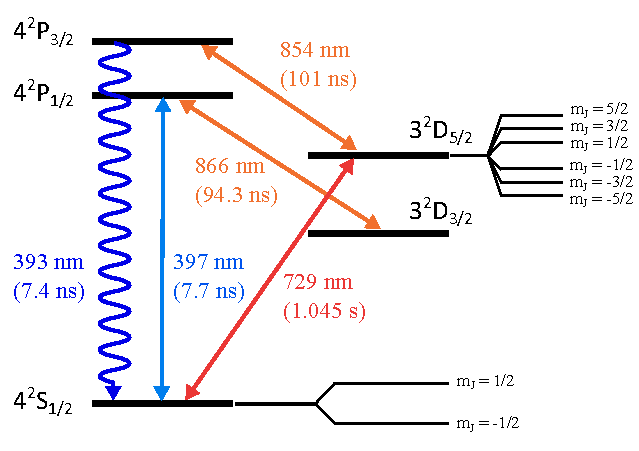
\includegraphics{figures/2/Fig_CaSpec}
        \caption{\label{fig:CaSpec} Level diagram of $^{40}$Ca$^+$ with relevant transitions shown (lifetimes in parentheses). Zeeman splitting is shown for the $S_{1/2}$ and $D_{5/2}$ levels and otherwise omitted. Data from \cite{James98.APB.66.181}.   }
    \end{center}
\end{figure}

The singly charged $^{40}$Ca$^+$ ion is well-researched for many quantum computing and quantum simulation applications \cite{Roos00.Thesis, Häffner2008155, Blatt2012, Schmidt03.Nature.422.408} and as a reference atom in optical atomic clocks \cite{ RevModPhys.87.637, Champenois2004298}. Among its most appealing features is that all of the relevant transitions for ionization, laser cooling, state preparation/detection, qubit operations, and frequency referencing are accessible via solid state laser sources. The level diagram of relevant transitions is shown in Fig. \ref{fig:CaSpec}; the transition wavelengths and lifetimes are summarized in Table \ref{table:CaTransitions} \cite{James98.APB.66.181}. A brief summary of their functions follows. Note that $^{40}$Ca$^+$ has no nuclear spin, and therefore $m_F = m_J$ for all transitions discussed. %The fine structure Zeeman splitting will be of interest to us in the $S_{1/2} \leftrightarrow D_{5/2}$ transition only.  % ; the Land\'{e} factors for these levels is given in Table \ref{table:CaLande} \cite{Roos00.Thesis}.

\begin{table}
\caption{Relevant transition wavelengths and lifetimes in $^{40}$Ca$^+$ \cite{James98.APB.66.181}}
\begin{center}

\begin{tabular}{|c|c|c|c|c|c|}
\hline
  & $S_{1/2} \leftrightarrow P_{1/2}$ & $D_{3/2} \leftrightarrow P_{1/2}$ & $D_{5/2} \leftrightarrow P_{3/2}$ & $S_{1/2} \leftrightarrow P_{3/2}$ & \\ \hline
$\lambda$ & 396.847 & 866.214 & 854.209 & 393.366 & nm \\ \hline
$\tau$ & 7.7 & 94.3 & 101 & 7.4  & ns \\
\hline
\end{tabular}

% table break
\begin{tabular}{c}
\\
\end{tabular}

\begin{tabular}{|c|c|c|}
\hline
 & $S_{1/2} \leftrightarrow D_{5/2}$ & \\ \hline
$\lambda$ & 729.147 & nm \\ \hline
$\tau$ & 1.045 & s \\
\hline 
\end{tabular}
\end{center}
\label{table:CaTransitions}
\end{table}  
%%%%%%%%%%%%
%\begin{table}
%\caption{Relevant Land\'{e} factors \cite{Roos00.Thesis}}
%\begin{center}

%\begin{tabular}{|c|c|c|}
%\hline
 % & $S_{1/2}$ & $D_{5/2}$ \\ \hline
%g_J & 2 & 6/5 \\ 
%\hline
%\end{tabular}
%\end{center}
%\label{table:CaLande}
%\end{table}  
\hfill
\noindent
\begin{flushleft}
\underline{$S_{1/2} \leftrightarrow D_{5/2}$ (729 nm)   }
\end{flushleft}  
This is the primary qubit and reference transition used in $^{40}$Ca$^+$ experiments. It is a quadrupole transition, unlike the rest of those described here (which are dipole), thus it has a suitably long lifetime ($\sim$1 s) for such purposes. Its $\sim$1 Hz natural linewidth also allows for resolution of all the trap secular modes in its spectroscopy. This makes it ideal for resolved sideband cooling, and for any quantum computing or simulation experiments which rely on sideband operations. The secular sidebands in the 729 nm transition are also used to measure the average number of quanta ($\bar{n}$) in their respective modes when the ion is in the Lamb-Dicke regime \cite{Turchette.PRA.61.063418}. 

\begin{figure}[t]
    \begin{center}
        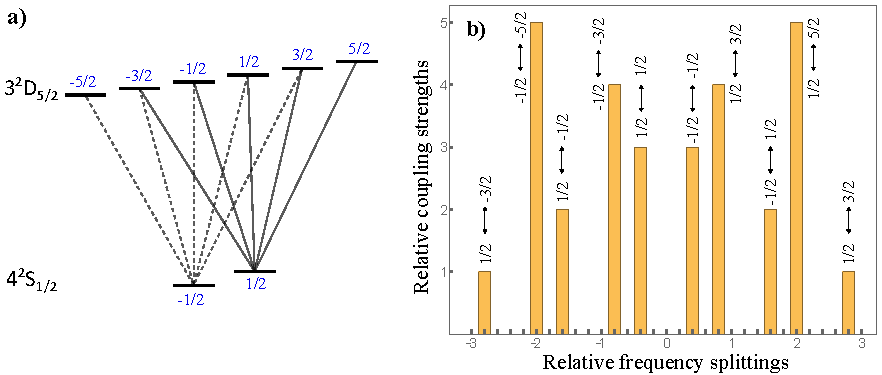
\includegraphics{figures/2/Fig_ZeemanSplits}
        \caption{\label{fig:ZeemanSplits} (a) Allowable transitions of the $S_{1/2} \leftrightarrow D_{5/2}$ quadrupole transition when the ion experiences a non-zero magnetic field. (b) Relative transition coupling strengths vs. relative frequency splittings in an arbitrary magnetic field. The coupling strengths here are dependent on respective Clebsch-Gordan factors. The total span of the frequency splittings is $\sim$ 34 MHz in our experiment, arising from a 4.3 G magnetic field.   }
    \end{center}
\end{figure}

In the presence of a non-zero magnetic field, the electronic states in $^{40}$Ca$^+$ will Zeeman-split into angular momentum states; $S_{1/2}$ and $D_{5/2}$ become $|S_{1/2}, m_J \rangle$ and $|D_{5/2}, m_J\rangle$ (Fig. \ref{fig:ZeemanSplits} (a)). The splittings will be proportional to the applied magnetic field $B$  \cite{Roos00.Thesis}:
\begin{equation}
\Delta E = g_J \ \mu_B \ m_J  B  \text{,}
\end{equation}
where $\mu_B$ is the Bohr magneton and $g_J$ is the Land\'{e} factor for each transition ($g_J = 2\text{,} \ (6/5)}$ for $S_{1/2}$ and $D_{5/2}$, respectively). There will subsequently be ten non-degenerate $|S_{1/2}, m_J \rangle \leftrightarrow |D_{5/2}, m_J\rangle$ transitions which satisfy the quadrupole selection rule $|\Delta m_J| = 0, 1, 2$  (Fig. \ref{fig:ZeemanSplits} (b)). Their relative coupling strengths $\Omega$ depend on respective Clebsch-Gordan factors; they can also be affected by the relative geometry between the magnetic field and the exciting laser's wavevector and polarization (this will be discussed in the next section). In our experiment, a 4.3 G field is sufficient to separate these transitions across a range of approximately 34 MHz. 
\hfill
\noindent
\begin{flushleft}
\underline{$S_{1/2} \leftrightarrow P_{1/2}$ (397 nm)   }
\end{flushleft}
The $S_{1/2} \leftrightarrow P_{1/2}$ transition at 397 nm is used for Doppler cooling, state preparation, and state detection of the ion(s). These functions will be discussed in Secs. 2.5 and 2.6. We detect fluorescence at this wavelength with a photo-multiplier tube (details in Ch. 3).
\hfill
\noindent
\begin{flushleft}
\underline{$D_{3/2} \leftrightarrow P_{1/2}$ (866 nm)   }
\end{flushleft}
Because the $P_{1/2}$ level decays undesirably to the metastable $D_{3/2}$ level approximately 6\% of the time \cite{Roos00.Thesis}, the $D_{3/2} \leftrightarrow P_{1/2}$ transition is continuously driven/repumped by an 866 nm laser in order to avoid population shelving.
\hfill
\noindent
\begin{flushleft}
\underline{$D_{5/2} \leftrightarrow P_{3/2}$ (854 nm)   }
\end{flushleft}
Because the metastable $D_{5/2}$ has a relatively long lifetime on the order of a second, the $D_{5/2} \leftrightarrow P_{3/2}$ transition is driven with an 854 nm laser in order to rapidly depopulate the $D_{5/2}$ state when desired. The short lifetime ($\sim$ 7 ns) of the $P_{3/2}$ state subsequently ensures a rapid return to the $S_{1/2}$ ground state.



\hfill
%%%%%%%%%%%%%
\section{Laser-ion interactions}

We will now discuss the fundamental principles of laser-ion interactions in the approximation of two-level systems. Our treatment follows those in Refs. \cite{Roos00.Thesis, Leibfried03.RMP.75.281}. 

\subsection{Basic interactions}
For a harmonically trapped ion, interacting with a traveling wave laser tuned near to a transition resonance, the corresponding Hamiltonian is
\begin{equation}
\begin{split}
H &= H_0 + H_i \\
H_0 &= \frac{p^2}{2 m} + \frac{1}{2} m \omega_i^2 x^2 + \frac{1}{2} \hbar \omega_0 \sigma_z \\
H_i &= \frac{1}{2} \hbar \Omega (\sigma_+ + \sigma_-) ( e^{i (kx - \nu t + \phi)} + e^{-i (kx - \nu t + \phi)} ) \text{,}	
\end{split}
\label{eq:basicH}
\end{equation}
where $\sigma_z$, $\sigma_+$, $\sigma_-$ are the Pauli spin matricies, $\omega_i$ is the motional frequency of the harmonic potential, $\omega_0$ is the transition frequency, $\Omega$ is the transition coupling strength (or Rabi frequency), $\nu$ is the laser frequency, and $k$ is the laser wavenumber. In this treatment we assume that the both the laser and harmonic oscillations are along the x-axis. The generalization to more dimensions and/or incident angles in the laser is straightforward. 

We can replace various terms in Eq. \ref{eq:basicH} with $a$ and $a^{\dagger}$, the creation and annihilation operators of the harmonic oscillator. Defining the Lamb-Dicke parameter
\begin{equation}
\eta = k \sqrt{ \frac{\hbar}{2 m \omega_i} }
\end{equation}
we get $kx = \eta (a + a^{\dagger})$, and obtain
\begin{equation}
\begin{split}
H_0 &= \hbar \omega_i (a^{\dagger} a + \frac{1}{2} ) + \frac{1}{2} \hbar \omega_0 \sigma_z \\
H_i &= \frac{1}{2} \hbar \Omega (\sigma_+ + \sigma_-) [ e^{i \eta (a + a^{\dagger}) } e^{-i \nu t} e^{i \phi}  +  e^{-i \eta (a + a^{\dagger}) } e^{i \nu t} e^{-i \phi} ]  \text{.}
\end{split}
\end{equation}
Transforming into the interaction picture $H_I = U_0^{\dagger} H U_0$, where $U_0 = exp[-(i / \hbar) H_0 t]$, and discarding the rapidly oscillating terms exp$[\pm i (\nu + \omega_0)]$ (i.e. making the \textit{rotating wave approximation}), we end up with an interaction Hamiltonian of the form 
\begin{equation}
H_I = \frac{1}{2} \hbar \Omega \big( \sigma_+ \ e^{ i \eta [a(t) + a^{\dagger}(t) ] } \ e^{- i \Delta t} \ e^{i \phi}  \big) + H.c. \text{,}
\end{equation}
where $\Delta = \nu - \omega_0$ and $a(t) = a e^{-i \omega_i t}$. This describes coupling between the states $|g, n\rangle$ and $|e, n'\rangle$, where $n$ is the vibrational quantum number and $\hbar (\omega_e - \omega_g) = \hbar \omega_0$. The pairing of the electronic states $|e\rangle$ and $|g\rangle$ with the motional states $|n\rangle$ can also be thought of in the classical sense: the ion, which is oscillating in the trap potential, experiences a frequency-modulated laser in its rest frame which is modulated at the trap frequency. This is the manifestation of secular sidebands in the ion's excitation spectra. If the laser is tuned such that $\nu - \omega_0 \approx m \omega_i$, i.e. onto a sideband, then the transitions $|g,n\rangle \leftrightarrow |e, n+m\rangle$ can be driven. If $\nu - \omega_0 \approx 0$ then the transition $|g,n\rangle \leftrightarrow |e, n\rangle$ will be made with no change in quantum number. We refer to this as the \textit{carrier} transition. Fig. \ref{fig:729spec} shows how these features arise in the $S_{1/2} \leftrightarrow D_{5/2}$ spectroscopy. 

\begin{figure}[t]
    \begin{center}
        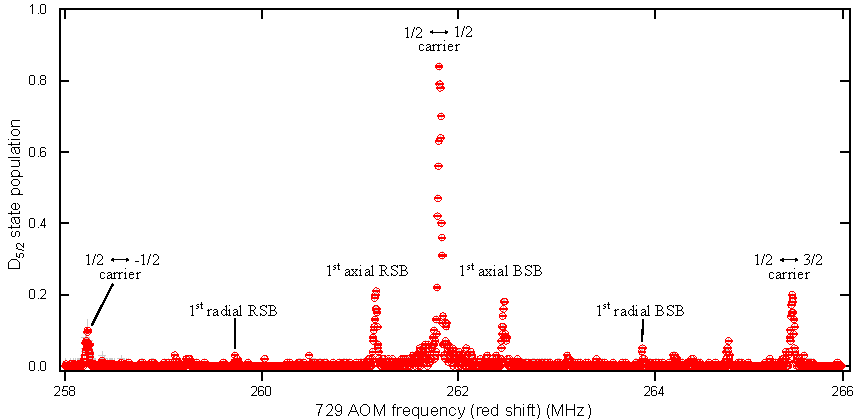
\includegraphics{figures/2/Fig_729spec}
        \caption{\label{fig:729spec} Sample spectroscopy data centered about the $|S_{1/2}, m_J = \frac{1}{2} \rangle \leftrightarrow |D_{5/2}, m_J = \frac{1}{2} \rangle$ carrier transition. Axial and radial sidebands on this transition are labeled. The frequency of the laser is being offset by an acousto-optic modulator (AOM).  }
    \end{center}
\end{figure}

\subsection{Time evolution}
The time evolution of the state $\psi (t) = \Sigma_n ( \ g_n (t) |g, n\rangle + e_{n+m} (t) |e, n + m\rangle \ )$ can be evaluated with the Schr\"{o}dinger equation $ i \hbar \partial_t \psi = H \psi$, which yields a set of coupled differential equations for $g_n (t)$ and $e_{n+m} (t)$. The general solution can be solved analytically as a 2x2 transformation matrix of the initial state vector:     
\begin{equation}
\begin{pmatrix} g_n (t) \\ e_{n+m,n}(t) \end{pmatrix} = T_n \begin{pmatrix} g_n (0) \\ e_{n+m,n} (0) \end{pmatrix} \text{,}
\label{eq:stateEvol}
\end{equation}
with
\begin{equation}
T_n = \begin{pmatrix} e^{-i \frac{\delta t}{2}} \big[ \cos (\frac{f_{n,m} t}{2}) + i \frac{\delta}{f_{m,n}} \sin (\frac{f_{n,m} t}{2}) \big ] & 
- 2 i e^{-i (\frac{\delta t}{2} \ - \frac{\pi |m|}{2} ) } \frac{\Omega_{n+m,m}}{f_{n,m}} \sin (\frac{f_{n,m} t}{2}) \\
 - 2 i e^{i (\frac{\delta t}{2} \ - \frac{\pi |m|}{2} ) } \frac{\Omega_{n+m,m}}{f_{n,m}} \sin (\frac{f_{n,m} t}{2}) &  
 e^{i \frac{\delta t}{2}} \big[ \cos (\frac{f_{n,m} t}{2}) - i \frac{\delta}{f_{m,n}} \sin (\frac{f_{n,m} t}{2}) \big ]
\end{pmatrix}
\text{.}
\label{eq:EvolMatrix}
\end{equation}
Here $\delta = ( \nu - \omega_0 ) - m \omega_i$ is the laser detuning from the $m$'th sideband, 
\begin{equation}
\Omega_{n+m, n} = \Omega \langle n + m | e^{ i \eta [a(t) + a^{\dagger}(t) ] } | n \rangle 
\label{eq:RabiFreq}
\end{equation}
is the scaled coupling strength, and $f_{n,m} = \sqrt{\delta^2 + \Omega_{n+m,n}^2}$ is the detuned frequency. 

We often consider the case with initial conditions $g_n (0) = 1$ and $e_{n+m} (0) = 0$ in Eq. \ref{eq:EvolMatrix}, i.e. the ion prepared initially in its ground state. In this case, the excited state population after a laser-ion interaction time $t$ is 
\begin{equation}
P_{e,n+m} (t) = | e_{n+m} (t) |^2 = \frac{ \Omega_{n+m, n}^2 }{ \delta^2 + \Omega_{n+m, n}^2 } \sin^2 \big( \frac{1}{2} \Omega_{n+m, n} t \big) \text{.}
\label{eq:numstatepop}
\end{equation}
This result characterizes the typical Rabi flopping scenario for driven excitations in a two-level system. 


\subsection{Lamb-Dicke regime approximations}
In the so called Lamb-Dicke regime, defined by ${\eta^2 (2n + 1) \ll 1}$, we can Taylor expand the exponential in Eq. \ref{eq:RabiFreq}:
\begin{equation}
e^{ i \eta [a(t) + a^{\dagger}(t) ] } \approx 1 + i \eta [a(t) + a^{\dagger}(t) ] + \mathcal{O}(\eta^2) \text{.}
\end{equation}
By making this approximation, we find (to lowest orders) explicit definitions of the coupling strengths for the carrier
\begin{equation}
\Omega_{car} = \Omega_{n,n} = \Omega \big[1 - \frac{\eta^2}{2}(1 + 2n) \big] \text{,}
\label{eq:Omega_car}
\end{equation}
the 1st order red sideband
\begin{equation}
\Omega_{rsb} = \Omega_{n-1,n} = \eta \sqrt{n} \ \Omega \ \text{,}
\label{eq:Omega_rsb}
\end{equation}
and the 1st order blue sideband
\begin{equation}
\Omega_{bsb} = \Omega_{n+1,n} = \eta \sqrt{n+1} \ \Omega \ \text{,}
\label{eq:Omega_bsb}
\end{equation}
which can be used in Eq. \ref{eq:numstatepop} for the respective excitations. In our configuration, $\eta \approx 0.07$ for a $(2 \pi) \times 1$ MHz trap frequency. This puts values of $n \lesssim 20$ safely within the Lamb-Dicke regime, which are routinely achievable with Doppler cooling techniques (see Sec. 2.5).


\subsection{Coupling strengths}
The analytical value of $\Omega$ depends on both the transition in question and the geometry of the experimental setup. For the $S_{1/2} \leftrightarrow D_{5/2}$ quadrupole transition, $H_i = \hat{Q} \Delta E(t)$ (i.e. the ion's quadrupole moment is coupled to the gradient of the electric field), and $\Omega$ becomes
\begin{equation}
\Omega =  \bigg| \frac{e E_0}{2 \hbar} \langle S_{1/2}, m_J | (\mathbf{\epsilon \cdot r})(\mathbf{k \cdot r}) | D_{5/2}, m_J' \rangle \bigg| \text{,}
\end{equation}
which is dependent on both the $m_J$ and $m_J'$ values in question (per Fig. \ref{fig:ZeemanSplits} (b)) and the relative geometry between the laser polarization $\mathbf{\epsilon}$, laser wavevector $\mathbf{k}$, and the applied magnetic field $\mathbf{B}$ \cite{James98.APB.66.181, Roos00.Thesis}. A full evaluation can be found in Ref. \cite{Roos00.Thesis}, but for our purposes it will suffice to consider two special cases: 1) $\mathbf{\epsilon}$, $\mathbf{k}$, and $\mathbf{B}$ are all mutually orthogonal, in which case only the $\Delta m = \pm 2$ transitions are coupled, and 2) $\mathbf{k}$ is at an angle $\phi = 45^o$ to $\mathbf{B}$ and $\mathbf{\epsilon}$ is orthogonal to their plane, in which case $\Delta m = 0$ transitions are strongly coupled, $\Delta m = \pm2$ transitions are weakly coupled, and $\Delta m = \pm1$ transitions are not coupled at all. We used the former configuration in the standing wave experiments (Ch. 4) and the latter configuration otherwise. 

In practice is often simplest to determine the coupling strengths empirically. For the $S_{1/2} \leftrightarrow D_{5/2}$ qubit/clock transition in $^{40}$Ca$^+$, a $\sim$ 10 mW resonant laser focused to a $\sim$ 30 $\mu$m waist gives $\Omega \approx$ 3 MHz in our system. This corresponds to a field strength $E_0 \approx 7 \times 10^4$ V/m at the beam center.

%\begin{align*}
%\Omega &=  \bigg| \frac{e E_0}{2 \hbar} \langle S_{1/2}, m_J | (\mathbf{\epsilon \cdot r})(\mathbf{k \cdot r}) | D_{5/2}, m_J' \rangle \bigg| \\
%&= \bigg| \frac{e E_0}{2 \hbar} \langle S_{1/2} || r^2 \mathbf{C}^{(2)} || D_{5/2} \rangle \mathlarger{\sum_{q=-2}^{2}} \begin{pmatrix}1/2 & 2 & 5/2 \\ -m_J & q & m_J' \end{pmatrix} %c_{ij}^{(q)} \epsilon_i n_j \bigg|
%\end{align*}


%%%%%%%%%%%%%%%%%%%%%%%%%%%%%%

\section{Thermal state distributions}

\begin{figure}[t]
    \begin{center}
        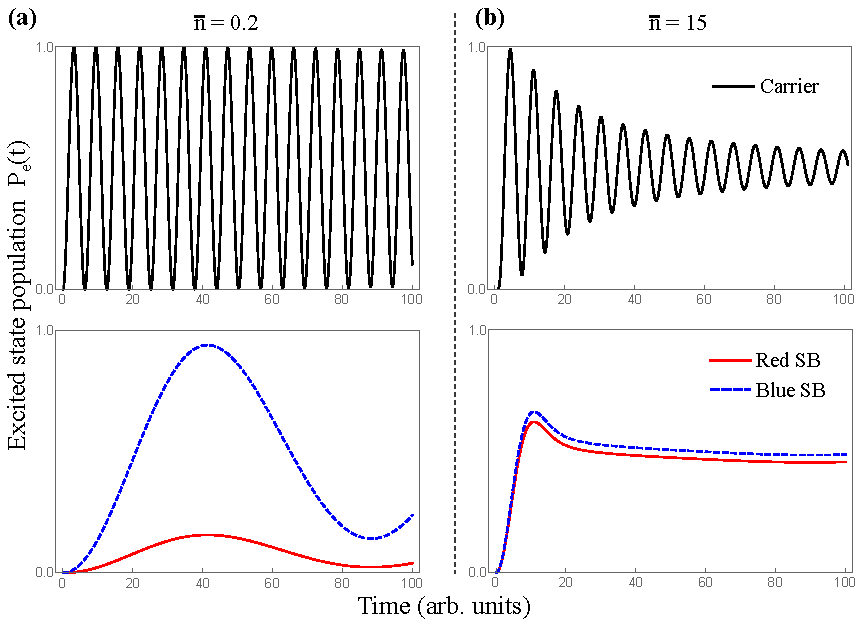
\includegraphics{figures/2/Fig_Flopping}
        \caption{\label{fig:flopping} Simulated carrier (top row) and red/blue sideband (bottom row) Rabi flops for (a) $\bar{n} = 0.2$ and (b) $\bar{n} = 15$, which are representative of our sideband cooled and Doppler cooled ions, respectively. These curves are calculated from Eq. \ref{eq:Pe} and Eqs. \ref{eq:Omega_car} - \ref{eq:Omega_bsb}, with $\delta = 0$. As $\bar{n}$ increases, the population inversion on the carrier loses contrast.  }
    \end{center}
\end{figure}

In practice, a trapped ion does not typically exist in a single number state (or Fock state) $| n \rangle$, but rather in a thermal distribution of number states defined by the probability distribution 
\begin{equation}
P_n (\bar{n}) = \frac{\bar{n}^n}{(\bar{n} + 1)^{n+1}}
\label{eq:Pn}
\end{equation}
where $\bar{n}$ is the average number of quanta in the thermal state \cite{Leibfried03.RMP.75.281}. Therefore, we can generalize Eq. \ref{eq:numstatepop} by summing over all number states. The overall excited state population $P_e (t)$ of the ion becomes 
\begin{equation}
\begin{split}
P_e (t) &= \mathlarger{\sum_{n=0}^{\infty}} \ P_n (\bar{n}) \ P_{e,n+m} (t) \\ 
&= \mathlarger{\sum_{n=0}^{\infty}} P_n (\bar{n}) \frac{ \Omega_{n+m, n}^2 }{ \delta^2 + \Omega_{n+m, n}^2 } \sin^2 \big( \frac{1}{2} \Omega_{n+m, n} t \big)
%(\bar{n}) \frac{ \Omega_{n+m, n}^2 }{ \delta^2 + \Omega_{n+m, n}^2 } \sin^2 \big( \frac{1}{2} \Omega_{n+m, n} t \big)
\label{eq:Pe}
\end{split}
\end{equation}
for a given thermal state characterized by $\bar{n}$. Note that a low value of $\bar{n}$ is necessary in order to achieve the maximum possible contrast in the population transfer (see Fig. \ref{fig:flopping}). Our Doppler cooled ions have $\bar{n} = 10-20$ (depending on various trap factors), which is generally sufficient for good contrast in a single excitation cycle; our sideband cooled ions have $\bar{n} \approx 0.1-0.2$, which is more than ideal. These cooling processes will be described in the next section. Fig. \ref{fig:flopping} shows how Eq. \ref{eq:Pe} evolves for the carrier and 1st order sidebands over this range of $\bar{n}$.


We measure $\bar{n}$ by driving the 1st order red and blue sidebands for a fixed interaction time $t$, and recording the ratio $R_k = (P_e^{rsb} / P_e^{bsb})$. This ratio is independent of $t$, and for thermal states is related to $\bar{n}$ by \cite{Turchette.PRA.61.063418}
\begin{equation}
\bar{n} = \frac{R_k}{1 - R_k} \text{.}
\label{eq:nbar}
\end{equation} 




%%%%%%%%%%%%%%%%%%%%%%%%%%%%%%

\section{Laser cooling techniques} 

We use two different methods of laser cooling to reduce the secular kinetic energy of our ions: Doppler cooling and resolved sideband cooling. We will summarize the basic principles here. Cooling is necessary not only for reaching the Lamb-Dicke regime, but for removing quanta that are continuously gained by the ion due to a variety of heating mechanisms. These include noise in the trap electrodes or external circuitry, noise in the RF drive signal, fluctuating patch potentials on the electrode surfaces, collisions with background atoms, etc \cite{Turchette.PRA.61.063418}. Ions that are not cooled will quickly gain enough energy to overcome the trap potentials, and will be lost.

\subsection{Doppler cooling}
Our description of Doppler cooling follows  Refs. \cite{Doppler, Leibfried03.RMP.75.281}. Doppler cooling is most easily modeled when considering the harmonic pseudopotential in one dimension, $V_{pp}(x) = \frac{1}{2} m \omega_x^2 x^2$\footnote{$V_{pp} = q \Phi_{pp}$.}. Assuming the ion's motion to be classical, then its velocity is given by
\begin{equation}
v(t) = v_0 cos(\omega_x t) \text{.}
\end{equation}
If we excite the ion to a state with an average lifetime $\tau$ that is much less than an oscillation period, then the ion's velocity is effectively constant throughout the cycle of absorption and spontaneous emission. This allows the average radiation pressure exerted by the exciting laser to be modeled as a continuous force dependent on the ion's velocity. 

In typical conditions, the average force can be linearized in $v$:
\begin{equation}
F_{ave} \approx F_0 (1 + \kappa v) \text{,}
\end{equation}
where $F_0 \propto \hbar k$, \footnote{If the exciting laser is at an angle $\theta$ to the ion's oscillation axis, then $k$ is simply replaced by $k \cos (\theta)$.} and $\kappa \propto \Delta = \nu - \omega_0$, with $\Delta$ being the laser detuning from resonance as before. The average change in energy of the ion over many oscillation periods can therefore be described as
%\begin{equation}
%\kappa = \frac{ 8 k \Delta / \Gamma^2 }{1 + 2( \Omega / \Gamma)^2 + (2 \Delta / \Gamma)^2 } \text{.}
%\end{equation}
%Here, $\Delta = \nu - \omega_0$ is the laser detuning from transition resonance, $\Gamma$ is the transition decay rate (or linewidth), and $\Omega$ is the on-resonance coupling strength. 
\begin{equation}
\frac{d E}{d t} = \langle F_{ave} v \rangle = F_0 \langle v \rangle + F_0 \kappa \langle v^2 \rangle = F_0 \kappa \langle v^2 \rangle \text{,}
\end{equation}
since $\langle v(t) \rangle = 0$. Because $\kappa \propto \Delta$, $( d E / d t )$ will be negative when $\Delta < 0$, and the ion will subsequently be cooled. At the same time, there will be some amount of heating present due to recoil from the emission cycles. Cooling will continue until equilibrium is reached between these two processes, which places a limit on the degree of cooling achievable. This limit is reached when the laser detuning is
\begin{equation}
\Delta = - \frac{\Gamma}{2} \sqrt{1 + 2 (\Omega / \Gamma)^2} \approx - \frac{\Gamma}{2} \text{,}
\end{equation}
where $\Gamma$ is the transition decay rate (or linewidth), $\Omega$ is the on-resonance coupling strength, and $\Gamma \gg \Omega$, generally. In practice the transition can be power-broadened beyond its natural linewidth $\Gamma$ by an intense enough laser, in which case it is sufficient to set $\Delta$ to approximately the FWHM value.

In our system we use the 397 nm laser to Doppler cool on the $S_{1/2} \rightarrow P_{1/2}$ transition, which has $\tau = 7.7$ ns and a corresponding linewidth $\Gamma \approx$ 20 MHz. We red-detune the laser by 10 MHz to achieve maximum cooling, which produces $\bar{n} = 10-20$ for a single ion (depending on trap factors such as stray fields). Doppler cooling is performed continuously when the ion is idle, simply by virtue of the laser being switched on. When cooling immediately before, during, or after an experiment, we use pulses that are $100 - 400$ $\mu$s in duration (depending on available beam power).   

\subsection{Sideband cooling}
To cool the ion(s) beyond the Doppler limit we must use resolved sideband cooling techniques. Detailed descriptions of these methods can be found in Refs. \cite{Leibfried03.RMP.75.281, Cirac92.PRA.46.2668, PhysRevA.20.1521, RevModPhys.58.699}. Sideband cooling is performed on transitions where $\Gamma \ll \omega_i$, i.e. when the transition linewidth is sufficiently narrow for the sidebands to be resolved. In this case, we can excite the transition directly on a red sideband (i.e. $|g,n\rangle \rightarrow |e, n+m\rangle$ for $m<0$) and subsequently reduce the vibrational quantum number. The 1st order red sideband ($m = -1$) is generally used since it couples most strongly. Each successive excitation on the 1st order red sideband removes an additional quanta, until the ion approaches its motional ground state. At this point, the average number of motional quanta $\bar{n}$ is approximately
\begin{equation}
\bar{n} \approx \frac{\Gamma^2}{4 \omega_i^2} \ \text{,} %\bigg[ \bigg(\frac{\tilde{\eta}}{\eta}\bigg)^2 + \frac{1}{4} \bigg] \text{,}
\end{equation}
where $\eta$ and $\tilde{\eta}$ are Lamb-Dicke factors associated with absorption and emission processes, respectively. %The bracketed term is of order unity, therefore $\bar{n} \ll 1$ since $\omega_i \ll \Gamma$. 
This is equivalent to the ion being in the ground state $|0\rangle$ with a probability very close to 1. 

When the red sideband transition is allowed to decay naturally via spontaneous emission, the cooling rate $R_n$ depends on both the decay rate $\Gamma$ and the red sideband coupling strength $\Omega_{rsb} = \eta \sqrt{n} \ \Omega$:
\begin{equation}
R_n = \Gamma \ \frac{(\eta \sqrt{n} \ \Omega)^2}{2(\eta \sqrt{n} \ \Omega)^2 + \Gamma^2} \text{.}
\end{equation}
This can be very slow, given that $\Gamma$ is often on the order of Hz, $\eta \ll 1$, and $n$ is continuously decreasing. It is possible to speed up this process by coupling the excited state to an auxiliary state with a much shorter lifetime. The effective decay rate $\tilde{\Gamma}$ becomes
\begin{equation}
\tilde{\Gamma} = \frac{\Omega_{aux}^2}{(\Gamma_{aux} + \Gamma)^2 + 4 \Delta_{aux}^2} \ \Gamma_{aux}
\end{equation}
and is adjustable via the coupling laser's power and detuning $\Delta_{aux}$. 

In our system we sideband cool on the 1st order red sideband of the $S_{1/2} \rightarrow D_{5/2}$ transition ($\Gamma \approx 1$ Hz), which is excited by the appropriately tuned 729 nm laser. Beginning with a Doppler cooled ion, we drive the $S_{1/2} \rightarrow D_{5/2}$ sideband on resonance for a time period $T_n = \pi / (\eta \sqrt{n} \Omega)$, assuming $n \approx 15$ intially. We then use 854 nm light to couple the $D_{5/2}$ state to the auxiliary $ P_{3/2}$ state, which subsequently decays back to the $S_{1/2}$ ground state on the order of nanoseconds. A $5-10$ $\mu$s pulse of 854 nm light at modest intensities is sufficient to clear the $D_{5/2}$ population. We repeat these steps 2 or 3 times since the population inversion on the red sideband transition is never complete (see Fig. \ref{fig:flopping}). The entire process is then repeated with an updated value of $T_n$, until we achieve measured values of $\bar{n} = 0.1-0.2$. 



%Every absorption/excitation event exerts a change in momentum $\Delta p = \hbar k \cos(\theta)$ upon the ion, where $\theta$ is the angle between the laser and the motional axis (for simplicity, we will assume $\theta = 0$). The rate of absorption-emission cycles is equal to $\Gamma \rho_{ee}$, where $\Gamma$ is the decay rate (or linewidth) of the transition and $\rho_{ee} = \langle e | \hat{\rho} | e \rangle$ is the density matrix element corresponding to the excited state probability. In this case, $\rho_{ee}$ is defined as
%\begin{equation}
%\rho_{ee} = \frac{s/2}{1 + s + [ 2 (\Delta - \mathbf{k \cdot v}) / \Gamma ]^2} \text{,}
%\end{equation} 
%where $s = 




%%%%%%%%%%%%%%%%%%%%%%%%%%%%%%%%%
\section{State preparation and detection}

\begin{figure}[t]
    \begin{center}
        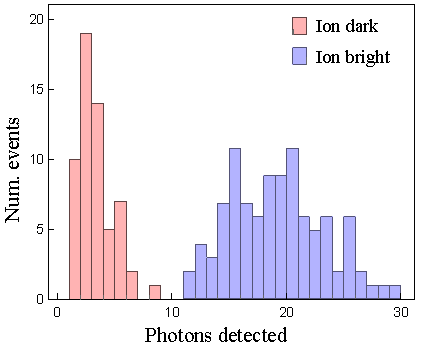
\includegraphics{figures/2/Fig_histograms}
        \caption{\label{fig:histograms} Example histograms for a ``dark'' and ``bright'' ion, which are either non-fluorescing or fluorescing, respectively, represented by the number of photons detected in a given detection time. So long as the respective distributions are distinguishable, then the number of photons detected during a detection event can be correlated to the ion's state (i.e. $S_{1/2}$ or $D_{5/2}$) at the time of measurement.}
    \end{center}
\end{figure}

During Doppler cooling, the spontaneous decay of the $P_{3/2}$ state will populate the $|S_{1/2}, m_J = \frac{1}{2} \rangle$ and $|S_{1/2}, m_J = -\frac{1}{2} \rangle$ states equally on average. Subsequently, any coherent excitation to a $|D_{5/2}, m_J \rangle$ state will achieve $\approx$ 50\% population inversion at best. To selectively prepare ion(s) in a single ground state Zeeman level, we pulse them with circularly polarized 397 nm light that is co-axial to the applied magnetic field. This couples only the $|S_{1/2}, m_J = \frac{1}{2} \rangle$ or $|S_{1/2}, m_J = -\frac{1}{2} \rangle$ level to the $P_{3/2}$ state, depending on whether the light is $\sigma_-$ or $\sigma_+$ polarized, and will depopulate that particular state over many cycles. We can state prepare either $m_J$ level to between 95-99 \% population (limited by the polarization optics and exact beam angle relative to $\mathbf{B})$. 

We also require a reliable method of measuring the ion's final state, i.e. measuring $P_e(t)$ in Eq. \ref{eq:Pe}, after performing coherent operations on the $S_{1/2} \rightarrow D_{5/2}$ transition. Pulsing the ion with the 397 nm laser projects it into into either the $S_{1/2}$ or $D_{5/2}$ state, with outcome probabilities $1 - P_e(t)$ and $P_e(t)$ respectively. The ion will then either fluoresce on the $S_{1/2} \leftrightarrow P_{1/2}$ transition in the former outcome, or remain dark in the latter. This is the so-called electron shelving method \cite{Roos00.Thesis, Leibfried03.RMP.75.281}. As long as the fluorescing ion produces enough photon counts on a detector to be distinguishable from dark/background (see Fig. \ref{fig:histograms}), then this process can be repeated until a suitable histogram of measurement outcomes is accumulated, providing a measured value of $P_e(t)$.  



%%%%%%%%%%%%%%%%%%%%%%%%%%%%%%%%%%
\section{Micromotion effects and compensation}

All of the theory and experimental details discussed here assume the ion is located on the RF null, and therefore neglect micromotion. If the ion is pushed off of the RF null by stray electric fields, or otherwise, then there can be significant issues. In particular, the linewidth of the 397 nm $S_{1/2} \leftrightarrow P_{1/2}$ transition becomes broadened and ``flattened'' as the micromotion modulation increases, since $\Gamma$ is on the order of $\Omega_{RF}$ in this case. This effectively cripples Doppler cooling, and makes state detection impossible since there is no longer a discernible resonance peak to distinguish a fluorescing ion from a dark one (i.e. the histograms in Fig. \ref{fig:histograms} cannot be discerned). By tuning the 397 nm laser to the red micromotion sideband (not the blue, since Doppler heating would occur when $\Delta > 0)$ and adjusting the ion's position until fluorescence is minimized, we can compensate for micromotion in the plane of the laser. Other methods of detecting and minimizing minimization exist, such as measuring average ion displacements as a function of trap potentials, or monitoring the amplitude of resolved sidebands, or using parametric excitations \cite{Berkeland98.JAP.83.5025, doi:10.1063/1.4930037}, but for our purposes the method described is sufficient.

Even when we make these compensations, non-trivial micromotion could still be occurring in the direction orthogonal to the plane of the laser. This can be problematic when measuring spectroscopy on a transition where $\Gamma \ll \Omega_{RF}$, as there will exist micromotion sidebands that are significantly removed in frequency relative to the transition's linewidth and the spread of its angular momentum states and secular sidebands. If the transition resonance frequencies are not already known, it can be easy to confuse a set of micromotion sideband spectra with the carrier spectra--a fact we learned during the course of these experiments. Deliberately displacing the ion from the RF null is a way to distinguish these features--if the coupling strengths get stronger, then they are micromotion sidebands. 

%%%%%%%%%%%%%%%%
% Chapter 3
%%%%%%%%%%%%%%%%

\chapter{Experimental configuration}



\section{The Gen IIc planar ion trap}
 
\begin{figure}[t]
    \begin{center}
        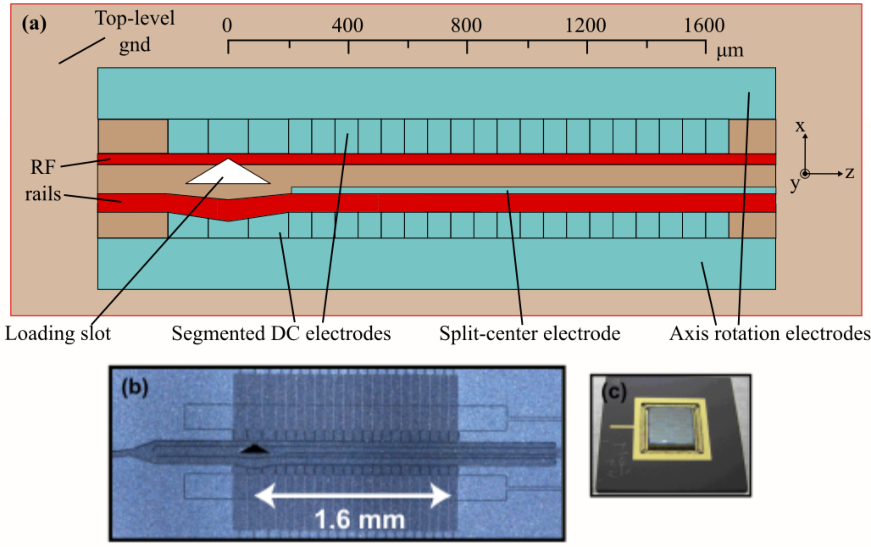
\includegraphics{figures/3/Fig_genIItrapR}
        \caption{\label{fig:genIItrap} Figures from Ref. \cite{IonTrap}. (a) Schematic view of the active trap region in the Gen IIc. (b) Optical microscope image of the active region. (c) The fabricated trap is mounted on a 100 pin CPGA for voltage control of the electrodes.   }
    \end{center}
\end{figure}

For all of the work described in this thesis we have used GTRI Gen IIc surface electrode linear ion trap (Fig. \ref{fig:genIItrap}), which transforms the linear RF trap geometry into a planar one. The design, fabrication, and performance characteristics of this trap are described in detail in Ref. \cite{IonTrap}.  The trap design is based on an asymmetric five-wire geometry \cite{FiveWire}. A pair of RF electrodes is combined with a split center DC electrode and segmented outer DC electrodes in order to provide the confining RF and DC potentials. The widths and placement of these electrodes have been chosen for a target ion height of 63 $\mu$m above the surface, and so that the radial axes are rotated approximately 20$^o$ relative to surface normal. The rotated axes allow for both radial secular modes to be Doppler cooled by a single laser parallel to the trap surface. Said modes have non-degenerate frequencies $\omega_{r1}, \ \omega_{r2} \approx (2 \pi) \times 4-6$ MHz, consistent with the values $q_i \approx 0.15$ and $a_i \approx 0.01$ which parameterize the trap. The exact frequencies vary based on factors such as stray field gradients and (as will be relevant in Ch. 4) the ion's position relative to the RF null. The single axial secular mode has a frequency $\omega_{z} \approx (2 \pi) \times 1$ MHz.

The DC segmented electrodes allow for axial transport of ions along the 1600 $\mu$m length of the active trapping region (Fig. \ref{fig:genIItrap} (a)). This is done with computer modeled sets of applied potentials on the electrodes which produce axial harmonic wells at regularly spaced intervals of around $\mu$m throughout the active region. These are referred to as the trap waveforms. Interpolation between adjacent waveforms provides harmonic wells at any position in the active region. Ion transport occurs by sequentially updating the electrodes in order to produce a moving harmonic well. Multiple wells can be generated to simultaneously trap multiple ions, as well as to merge/separate them into/from a linear chain in a single harmonic potential. Chains of 10 ions have previously been demonstrated in our trap \cite{IonTrap}. In addition, the waveforms can generate static offset fields from the electrodes which shift the ions' radial position by up to 10 $\mu$m. This used primarily for the compensation of stray electric fields which push the ion away from the RF null and increase micromotion, but can also be utilized for experimental purposes as we will see in Ch. 4.

Ion capture occurs at the location of the backside loading slot, defined as position z = 0 $\mu$m on the trap axis. A flux of neutral atoms is ejected from a coil-heated sample of material and passes through the slot. The neutral atoms are then ionized using a resonance enhanced two-photon scheme \cite{Gulde2001}, in which a resonant 423 nm laser interaction is followed by a 377 nm laser interaction, with the two lasers overlapping at the loading position. Harmonic well depths of several eV are suitable for capturing ions from the flux. 

\begin{figure}[t]
    \begin{center}
        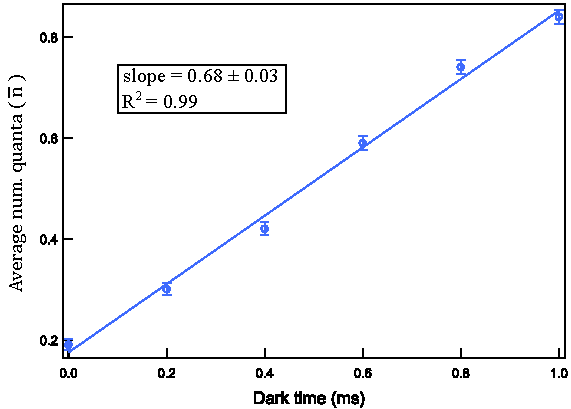
\includegraphics{figures/3/Fig_HeatingRate}
        \caption{\label{fig:heatingrate} Heating rate data for our trap: $\bar{n}$ vs. ``dark time'' (during which the ion is not actively cooled). The fitted slope gives the heating rate for our trap as $\dot{\bar{n}} \approx 680$ quanta/sec. The heating rate was measured on the 1.3 MHz axial mode. }
    \end{center}
\end{figure}


As mentioned in Sec. 2.5, heating of ions will occur due to electric field noise, fluctuating patch potentials of electrodes, etc. All traps have an inherent heating rate $\dot{\bar{n}}$ which is approximately linear in time near the ground state. By measuring $\bar{n}$ as a function of time without active cooling (``dark time''), we can determine the heating rate. In our trap we measure $\dot{\bar{n}} \approx$ 680 quanta/s on the 1.3 MHz axial mode (see Fig. \ref{fig:heatingrate}). For comparison, heating rates in similar traps are typically in the $10^2 - 10^3$ quanta/s range \cite{doi:10.1063/1.4917385, PhysRevLett.96.253003, PhysRevA.76.033411, Shu14.PRA.89.062308}.

%%%%%%%%%%%%%%%%%%%%%%%%%%%%%%
\section{Trap enclosures and fluoresence detection}

\begin{figure}[t]
    \begin{center}
        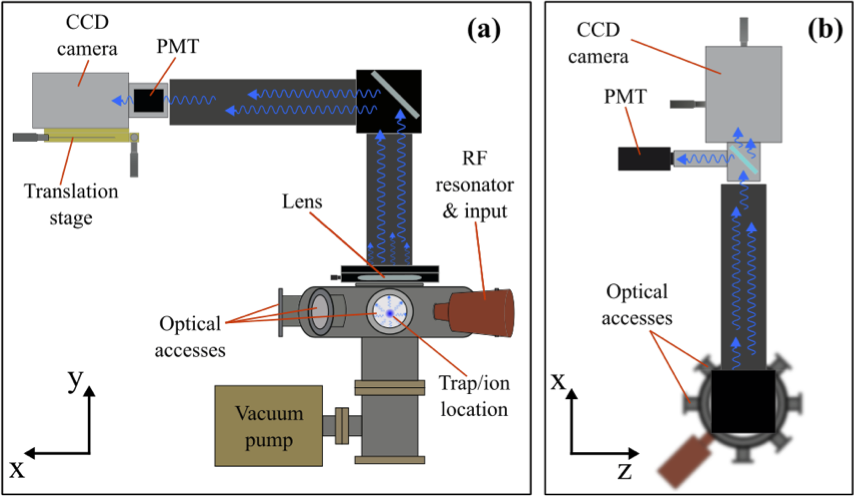
\includegraphics{figures/3/Fig_CameraConfigPNG}
        \caption{\label{fig:CameraConfig} Illustrated schematic of the trap's vacuum enclosure and fluoresence detection optics, in a (a) side-on and (b) top-down perspective. Description in text.   }
    \end{center}
\end{figure}


Fig. \ref{fig:CameraConfig} shows an illustrated schematic of the trap enclosure and fluorescence detection optics. The fabricated Gen IIc trap is mounted on a CPGA chip (Fig. \ref{fig:genIItrap} (c)) and enclosed in stainless steel vacuum chamber held at $\sim 10^{-12}$ torr. The circular chamber has 7 optical access windows positioned at $45^{\circ}$ intervals about its center (more detail can be seen in Fig. \ref{fig:LaserConfig}). A large top-view window allows the trap surface to be continuously imaged by a CCD camera. The optical pathway of this camera is optimized to provide a $\sim 500 \times 500$ $\mu$m$^2$ viewing area when filtered to collect 397 nm light. Ion fluorescence at 397 nm occurs any time the ion interacts with the 397 nm laser. For high speed and high fidelity state detection, a portion of this light is directed onto a photomultiplier tube (PMT) which returns photon-count measurements back to the experiment control software. The camera and PMT are mounted together on a translation stage, allowing the entire length of the trap to be imaged. 

The entire configuration is enclosed in a magnetic shielding box with a removable front lid for access. Magnetometer measurements near the trap chamber record a factor of $\sim$ 5 reduction in ambient magnetic field noise when the lid is on and the trap chamber is fully shielded. All of the experiments in this thesis were run with full shielding. 



%%%%%%%%%%%%%%%%%%%%%%%%%%%%%%
%\section{Fluorescence detection}





%%%%%%%%%%%%%%%%%%%%%%%%%%%%%%
\section{Laser hardware and trap-side configuration}

\begin{figure}[ht]
    \begin{center}
        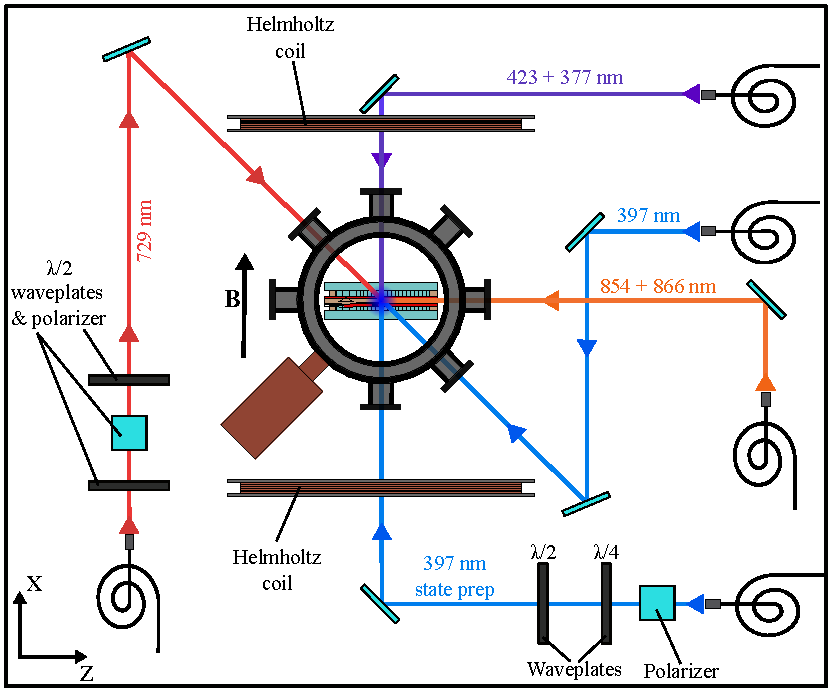
\includegraphics{figures/3/Fig_lasers5}
        \caption{\label{fig:LaserConfig} Illustrated schematic of the laser and magnetic field generation configuration at the trap chamber (trap not to scale). Fiber optic cables (black coils) bring appropriately conditioned light to the trap. A pair of Helmholtz coils produces a 4.3 G magnetic field in the $x$ direction. The 729 nm beam and 397 nm Doppler cooling beam are brought in at a 45$^{\circ}$ angle to the trap axis in order access/cool all secular modes. The 397 nm state preparation beam is coaxial with the $\mathbf{B}$ field. Beams pass through appropriate polarization optics when necessary. }
    \end{center}
\end{figure}

All of the laser wavelengths used in these experiments were generated with commercially available solid-state diodes and peripheral hardware. The 397, 423, 854, and 866 nm lasers are frequency stabilized to a rubidium reference source via a low finesse ($F \sim 150-200$) transfer cavity \cite{doi:10.1063/1.2337094}. The 729 nm laser is frequency stabilized in an ultra-low expansion (ULE) glass cavity via the Pound-Drever-Hall method \cite{doi:10.1119/1.1286663}. At the time of the experiments discussed in Ch. 4, the ULE cavity being used had a finesse $F \sim 10,000$ and stabilized the 729 nm linewidth to approximately 1-2 kHz. Since then it has been replaced by an $F \sim 150,000$ ULE cavity which is capable of stable linewidths in the range of 10-100 Hz.  

Frequency control of the 423 and 866 nm lasers is achieved by adjusting their stabilization set point in the transfer cavity. These beams are generally set before experiments and otherwise left static. For the 397, 729, and 854 nm beams we require dynamic control over the frequency during experiments, as well as rapid on-off switching. Both of these needs are met with Brimrose brand acousto-optical modulators (AOMs) which diffract and frequency-shift the beams with oscillating crystals. By changing the RF frequencies which drive the crystals we subsequently shift the diffracted laser frequencies, and by switching the RF drive signal on or off entirely with TTL electronics we obtain on-off control of our diffracted beams as well. The AOMs have -3 dB bandwidths typically in the 100 MHz range, and offer fast ramp-up and ramp-down times of $\sim$ 10 ns for beam switching purposes. The RF driving fields for the 397 and 729 nm beams are sourced from digital signal generators (more on these in the next section), and are amplified, TTL-switched, and otherwise modulated when necessary by Minicircuits components, primarily. 
The 397 nm beams--one for Doppler cooling and state detection, and a second for state preparation--and the 729 nm beam are in the double-pass configuration through their respective AOMs. The 854 nm beam is single-passed.

All of the appropriately conditioned light is brought to the trap chamber region via fiber-optic cables. Fig. \ref{fig:LaserConfig} shows the laser configuration entering the trap chamber. The 397 nm Doppler cooling and state detection light light is brought in at a 45$^{\circ}$ angle to the trap axis in order cool all secular modes. The state preparation 397 nm beam passes through a polarizer, a $\lambda/2$ waveplate, and $\lambda/4$ waveplate for circular polarization. The 729 nm beam passes through two $\lambda/2$ waveplates and a polarizer for optimal linear polarization, and is also incident at 45$^{\circ}$ to access all secular modes. Repump light at 854 and 866 nm is coaxial to the trap axis, and the 377 and 423 nm ionization beams are positioned at the loading slot. 

A pair of Helmholtz coils driven by a stable current source produce the 4.3 G magnetic field at the trap location. The current source is stable to within 10 $\mu$A.   


%%%%%%%%%%%%%%%%%%%%%%%%%%%%%%
\section{Signal generation, voltage control, and control software}

The RF signals which drive the AOMs for the 397 nm cooling and 729 nm beams are generated by Analog Devices AD9910 direct digital synthesizer (DDS) cards, which synchronized to a 1 GHz analog signal. These are controlled by a Xilinx XC6SLX45T-2 field programmable gate array (FPGA) device which has a 500$+$ MHz clock speed. The FPGA also controls the analog TTL signals for AOM switching, and accepts serial input signals from the PMT which correspond to photons detected. The RF signals for the 397 nm state preparation and 854 nm AOMs do not need to be updated quickly, and are therefore sourced from simple USB based devices.

DC voltages on the trap electrodes are controlled via National Instruments digital-to-analog converters which can be updated at rates of 10 kHz. They are low-pass filtered to reduce higher frequency noise. The electrode voltages reach the trap chip via access pins built into the vacuum chamber. The trap's RF drive frequency is sourced from a Hewlett-Packard analog signal generator and is amplified via a Minicircuits amplifier. The RF signal enters the trap chamber through a helical resonator, which maximizes the drive voltage on the trap surface while reducing noise \cite{Siverns2012}. Our trapping frequency $\Omega_{RF} = 52.525$ MHz is set to the resonance of the resonator. 

We use the Wavemetrics Igor software environment to control relevant hardware, run experimental procedures, and collect data. Experiments are triggered by a 60 Hz pulse sourced from the power mains in order to avoid sampling the AC magnetic field fluctuations. 



%%%%%%%%%%%%%%%%
% Chapter 4
%%%%%%%%%%%%%%%%

\chapter{Standing wave gate beams for coupling strength modulation}

In this chapter we will discuss experiments with standing wave laser fields and how the coupling strengths of carrier and sideband transitions may be controlled in our configuration. The results of this chapter were presented in Physical Review A \cite{StandingWave}.   

\section{Carrier and sideband coupling strengths in standing wave fields}

\begin{figure}[t]
    \begin{center}
        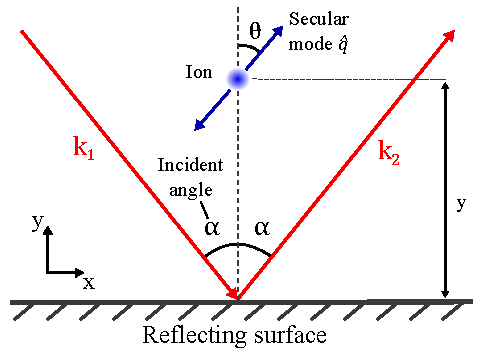
\includegraphics{figures/4/Fig_SWgeometry2}
        \caption{\label{fig:SWgeometry} Basic geometry of our standing wave configuration. An incident beam $\mathbf{k_1}$ at angle $\alpha$ w.r.t. surface normal is reflected, producing a second beam $\mathbf{k_2}$. The ion oscillates on a secular mode at angle $\theta$ w.r.t. the surface normal; its equilibrium height above the surface is $y$.   }
    \end{center}
\end{figure}

Here we will follow Sec. 2.3 and derive carrier and 1$^{st}$ order sideband coupling strengths for an ion interacting with two individual running-wave fields--one incident and one reflected from a nearby surface. Fig. \ref{fig:SWgeometry} illustrates the basic geometry in this situation. The incident and reflected beams $\mathbf{k_1}$ and $\mathbf{k_2}$ are each at an angle $\alpha$ with respect to the surface normal, and $|k_1| = |k_2| = k$. The ion's secular mode of interest oscillates with frequency $\omega$ at an angle $\theta$ with respect to the surface normal. The ion's mean height above the reflecting surface is given by $y$. For simplicity we will assume that the incident beam and secular axis are coplanar. 

The ion's motion in the $xy$ plane is described with the position operators $\hat{x}' = \hat{x}$ and $\hat{y}' = y + \hat{y}$. If $\hat{q}$ is the position operator corresponding to the ion's secular axis, then we have
\begin{equation}
\begin{split}
\hat{x}' &= \hat{q} \sin \theta \\
\hat{y}' &= y + \hat{q} \cos \theta \text{.}
\end{split}
\end{equation}
The ion's Hamiltonian per Eq. \ref{eq:basicH} will contain a term $\hat{H}_i$ for each beam:
\begin{equation}
\begin{split}
\hat{H}&_{i,1} = \frac{1}{2} \hbar \Omega_1 (\sigma_+ + \sigma_-) ( e^{i (\mathbf{k_1} \cdot \mathbf{\hat{r}} } e^{-i (\nu t - \phi)} + e^{-i (\mathbf{k_1} \cdot \mathbf{\hat{r}} } e^{i (\nu t - \phi)} ) \\
\hat{H}&_{i,2} = \frac{1}{2} \hbar \Omega_2 (\sigma_+ + \sigma_-) ( e^{i (\mathbf{k_2} \cdot \mathbf{\hat{r}} } e^{-i (\nu t - \phi)} + e^{-i (\mathbf{k_2} \cdot \mathbf{\hat{r}} } e^{i (\nu t - \phi)} ) \\
\hat{H}&_i = \hat{H}_{i,1} + \hat{H}_{i,2}  \text{,}
\end{split}
\label{eq:His}
\end{equation}  
where $\Omega_1$ and $\Omega_2$ are the respective coupling strengths in each interaction. The different coupling strengths arise from the differences in field strength between the two beams at the ion's position--this can be due to imperfect reflectivity from the surface, scattering of the reflected beam from surface features, varying intensities in the Gaussian beam shapes, or some combination thereof. The terms $\mathbf{k_1} \cdot \mathbf{\hat{r}}$ and $\mathbf{k_2} \cdot \mathbf{\hat{r}}$ in $H_i$ can be expressed as 
\begin{equation}
\begin{split}
\mathbf{k_1} \cdot \mathbf{\hat{r}} =& \ k \cos \alpha (-\hat{y}') + k \sin \alpha (\hat{x}') \\
=& -k y \cos \alpha + [ \sin \theta \sin \alpha - \cos \theta \cos \alpha ] k \hat{q} \\
\mathbf{k_2} \cdot \mathbf{\hat{r}} =& \ k \cos \alpha (\hat{y}') + k \sin \alpha (\hat{x}') \\
=& \ k y \cos \alpha + [ \sin \theta \sin \alpha + \cos \theta \cos \alpha ] k \hat{q} \text{.}
\end{split}
\label{eq:kdotr}
\end{equation}

Transforming now into the interaction picture $\hat{H}_I = \hat{U}_0^{\Dagger} \hat{H} \hat{U}_0$ as before, and making the substitutions in Eq. \ref{eq:kdotr} as well as $\gamma =( k y \cos \alpha )$ and $\hat{q} = \sqrt{\hbar / (2 m \omega)} (\hat{a} + \hat{a}^{\dagger})$, we obtain 
\begin{equation}
\begin{split}
\hat{H}_I = \frac{\hbar}{2} \hat{\sigma}_+ e^{-i (\Delta t - \phi) } \bigg\{& \ \Omega_1 \text{exp} \big[ -i \gamma + i \eta_1 ( \hat{a}(t) + \hat{a}^{\dagger}(t) ) \ \big] \\ 
+& \ \Omega_2 \text{exp} \big[ \ i \gamma + i \eta_2 ( \hat{a}(t) + \hat{a}^{\dagger}(t) ) \ \big] \bigg\} + \text{H.c.} \text{,}
\end{split}
\label{eq:HintSW}
\end{equation}
where $\eta_1$ and $\eta_2$ define respective Lamb-Dicke factors for each of the two beams:
\begin{equation}
\begin{split}
\eta_1 &= k \sqrt{ \frac{\hbar}{2 m w} }  [ \sin \theta \sin \alpha - \cos \theta \cos \alpha ] \\
\eta_2 &= k \sqrt{ \frac{\hbar}{2 m w} }  [ \sin \theta \sin \alpha + \cos \theta \cos \alpha ] \text{.}
\end{split}
\label{eq:etaSW}
\end{equation}
The coupling strength for the $|g,n\rangle \leftrightarrow |e,n+m\rangle$ transition becomes
\begin{equation}
\begin{split}
\Omega_{n+m, n} =& \ \Omega_1 e^{-i \gamma} \langle n + m | e^{ i \eta_1 ( \hat{a}(t) + \hat{a}^{\dagger}(t) ) } | n \rangle \\
+& \ \Omega_2 e^{i \gamma} \langle n + m | e^{ i \eta_2 ( \hat{a}(t) + \hat{a}^{\dagger}(t) ) } | n \rangle 
\label{eq:swRabiFreq}
\end{split}
\end{equation}
Making the Lamb-Dicke regime approximation once again, we can now find definitions for the carrier and sideband coupling strengths in the two-beam configuration:
\begin{equation}
\begin{split}
\Omega_{car} = \ &\Omega_1 e^{-i \gamma} \bigg[1 - \frac{\eta_1^2}{2}(1 + 2n) \bigg] + \Omega_2 e^{i \gamma} \bigg[1 - \frac{\eta_2^2}{2}(1 + 2n) \bigg] 
\label{eq:OmegaCarSW}
\end{split}
\end{equation}
and
\begin{equation}
\begin{split}
\Omega_{rsb} &= \sqrt{n} \ \big( \Omega_1 e^{-i \gamma} \eta_1 + \Omega_2 e^{i \gamma} \eta_2 \big) \\
\Omega_{bsb} &= \sqrt{n+1} \ \big( \Omega_1 e^{-i \gamma} \eta_1 + \Omega_2 e^{i \gamma} \eta_2 \big) \\ \text{.}
\end{split}
\label{eq:OmegaSbSW}
\end{equation}

Interference between the $e^{\pm i \gamma}$ terms produces fringes in the coupling strengths as the ion's equilibrium position $y$ changes. When $\cos \theta \cos \alpha > \sin \theta \sin \alpha$, $\eta_1$ and $\eta_2$ have opposite sign, and the carrier and sideband fringes are 180$^o$ out of phase. The $\gamma = k y \cos \alpha$ term represents the optical phase of the standing wave field which results from the mixing of beam components $k_{1,y} = - k \cos \alpha$, $k_{2,y} = k \cos \alpha$. When the ion's position coincides with a node of the standing wave, $\gamma = l \pi$ (with $l$ an integer), and $\Omega_{car}$ is maximized while $\Omega_{rsb}$ and $\Omega_{bsb}$ are minimized. On an antinode, $\gamma = (l + 1/2) \pi$, and the converse is true. In between the nodes and antinodes there will be a mixture of both carrier and sideband coupling. This node/antinode behavior refers to the case of a quadrupole transition; the behavior will be reversed for a dipole transition.

Achieving complete suppression requires $\Omega_1 = \Omega_2$ and $\alpha = 0$. If $\Omega_1 \neq \Omega_2$, then the field strengths $E_0$ of the incident and reflected beams are unequal at the ion's position, leading to some amount of residual running-wave light in the $y$ direction that will excite the ion indifferently. If $\alpha \neq 0$ then the same thing occurs, with the residual light propagating parallel to the trap surface in this case. \footnote{It is possible to completely suppress just the sidebands in the $\alpha \neq 0$ case, provided that the plane of the incident/reflected beams is orthogonal to the plane of the ion's oscillation axis, or alternatively if $\theta = 0$.}  


%%%%%%%%%%%%%%%%%%%%%%%%%%%%%%%%%
\section{Experimental realization}

\begin{figure}[t]
    \begin{center}
        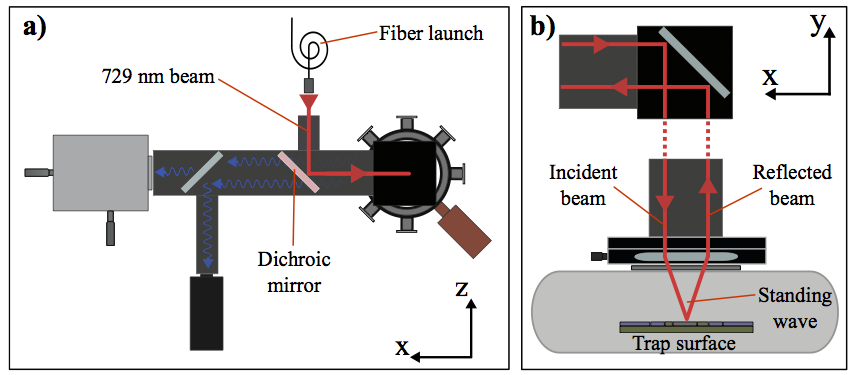
\includegraphics{figures/4/Fig_SWlaserConfigPNG}
        \caption{\label{fig:SWlaserConfig} (a) Top-down and (b) side-on views of the 729 nm laser configuration in this experiment. To achieve normal incidence of a 729 beam onto our trap surface, we use a dichroic mirror to introduce the beam into the optical path of our camera and PMT (see Sec. 3.3 and Fig. \ref{fig:CameraConfig}). By steering the incident beam and viewing the reflected beam's return path, we have minimized the incident angle depicted in (b) as much as possible.    }
    \end{center}
\end{figure}


The Gen IIc trap has a patterned aluminum surface which reflects 729 nm light with an 86\% reflectivity. We can therefore use the trap surface itself as the reflecting mirror for a standing wave field. This has the advantage of requiring no additional optics, save for those which steer the incident beam. As an added advantage, the ''mirror'' in this scenario will always remain a constant distance away from the ion, eliminating any concern of phase fluctuations in the field arising from microscopic movements of the mirror. Using a dichroic filter, we introduced a 729 nm beam into the optical path of the CCD camera and detection PMT in our setup. Fig. \ref{fig:SWlaserConfig} illustrates the configuration. Upon passing through the focusing lens for the camera/PMT (Fig. \ref{fig:SWlaserConfig} (b)), the beam is incident on the trap surface at an angle $\alpha \approx 20^o$. By steering the incident beam and viewing the reflected beam on its return path we were able to minimize this angle to the best of our ability. 

We excited ions on the $|S_{1/2}, m_J = -\frac{1}{2} \rangle \rightarrow |D_{5/2}, m_J = -\frac{5}{2} \rangle$ carrier transition in this experiment. Sideband excitations were performed on the radial mode with $\nu=2\pi \times 4.75$ MHz (on the RF null) and $\theta = 13^{\circ}$. Doppler cooling was done before every interaction, whereas sideband cooling was withheld in order to preserve enough quanta for appreciable sideband coupling strengths. To displace an ion's equilibrium position along the standing wave axis, we apply a static offset field $E_y$ through suitable adjustments to the trap's waveforms and potentials, as described in Sec. 3.1. The case $E_y$ = 0 corresponds to the ion being on the RF null. For $E_y>0$ and $E_y<0$, the ion is displaced along $+y$ and $-y$, respectively. The range of $E_y$ values used in this experiment displaces the ion over a 10 $\mu$m range. %The fringes in the carrier and sideband transitions resulting from this displacement are evident in Fig.~\ref{fig:EyScan}.

Displacing the ion from its equilibrium position on the RF null introduces micromotion, which will affect the dynamics in several ways beyond the coupling strength fringing. First, there will be an additional modulation to both the carrier and sideband coupling strengths \cite{Berkeland98.JAP.83.5025}. To account for this modulation, we multiply Eqs. \ref{eq:OmegaCarSW} and \ref{eq:OmegaSbSW} by the Bessel function $J_0(\kappa)$, where $\kappa$ is the modulation parameter given by
\begin{equation}
\label{eq:kappa}
\kappa = \cos \beta \frac{2}{\lambda\, \Omega_{RF}} \sqrt{ \frac{V_{pp}(x,y)}{m}  } .
\end{equation}
Here $\lambda = 729$ nm, $V_{pp}(x,y)$ is the RF pseudopotential, and $\beta$ is the angle between the micromotion direction and the standing wave axis.  Second, the ion's secular frequencies change depending on its position within the RF field. We account for this simply by measuring the sideband resonance at various displacements and parameterizing the results.

We can minimize micromotion in the $x$ direction by applying a static field $E_x$, suitably proportional to $E_y$, in order to displace the ion an angle which is twice that of the RF quadrupole axis. Along this trajectory the ion will experience only vertical RF field vectors (see Fig. \ref{fig:quadrupole}). Restricting the micromotion to the $y$ dimension is equivalent to choosing $\beta = 0$ in Eq. \ref{eq:kappa}.

\begin{figure}[t]
    \begin{center}
        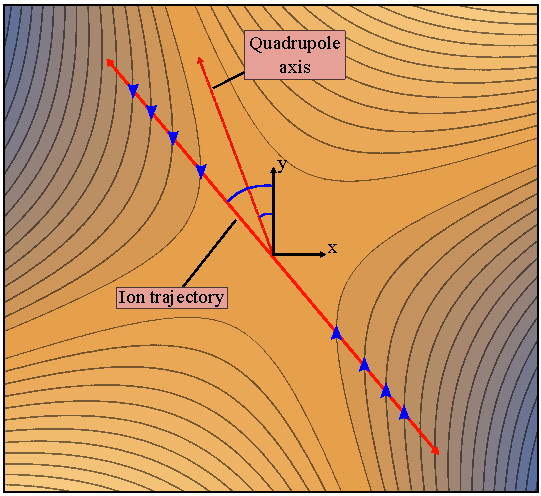
\includegraphics{figures/4/Fig_Quadrupole}
        \caption{\label{fig:quadrupole} Illustration of field vectors in a rotated quadrupole field. By displacing the ion at an angle which is twice that of the quadrupole axis, it will encounter field vectors that are only in the $\pm y$ direction (blue arrows). As such, horizontal micromotion will be minimized.  }
    \end{center}
\end{figure}






%%%%%%%%%%%%%%%%%%%%%%%%%%%%%%%%%
\section{Results}


\subsection{Coupling strength fringing and suppression}


\begin{figure*}
    \begin{center}
        %\makebox[\textwidth][c]{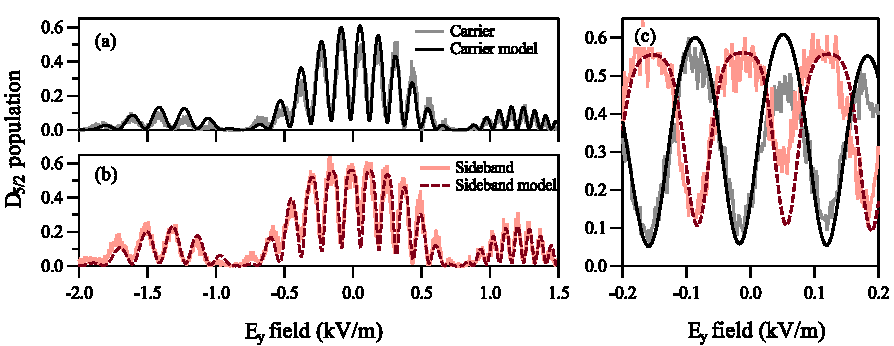
\includegraphics[width=1.2\textwidth]{figures/4/Fig_fringes3}}
        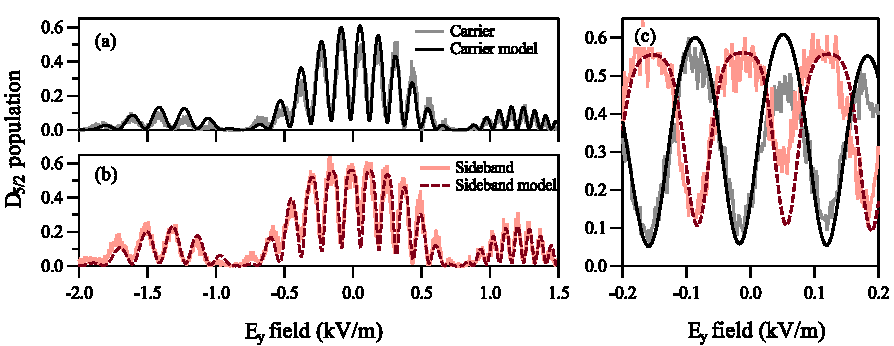
\includegraphics{figures/4/Fig_fringes3}
        \caption{\label{fig:fringes} $D_{5/2}$ populations vs. applied $E_y$ field measured after (a) carrier and (b) red sideband transitions. The sideband's gate beam power is 9.5~dB greater than the carrier's, and the interaction time is fixed for both cases (13~$\mu$s).  The overall envelope is generated by the micromotion modulation $J_0(\kappa)$ (see text). (c) The carrier and sideband populations oscillate 180$^o$ out of phase as the ion is transported through the standing wave fringes. The solid lines represent a fit to the data using the model described in the text. The deviation between the data and fit at $E_y\approx0.05$~kV$/$m may be due to scattering of the reflected light from the trap surface.}
    \end{center}
\end{figure*} 



Figs. \ref{fig:fringes} (a) and (b) show $D_{5/2}$ state populations measured after driving carrier or red sideband transitions as a function of applied $E_y$ field. The laser interaction time was fixed for all excitations (13 $\mu$s), and the power was set 9.5 dB greater for the sideband interactions in order to achieve an approximately equal population inversion. As can be seen in Fig. \ref{fig:fringes}, we observe the predicted fringing due to the standing wave field's phase, which are superimposed with the $J_0(\kappa)$ envelope resulting from micromotion modulation. Per Eqs. \ref{eq:OmegaCarSW} and \ref{eq:OmegaSbSW}, the maxima of the carrier fringes correspond to the ion positioned on nodes of the standing wave, whereas the minima correspond to antinodes. The carrier and sideband fringes are overlaid in Fig. \ref{fig:fringes} (c), demonstrating the 180$^{\circ}$ phase difference which occurs when the condition $\cos \theta \cos \alpha > \sin \theta \sin \alpha$ is met.



\begin{figure}[tbh]
    \begin{center}
        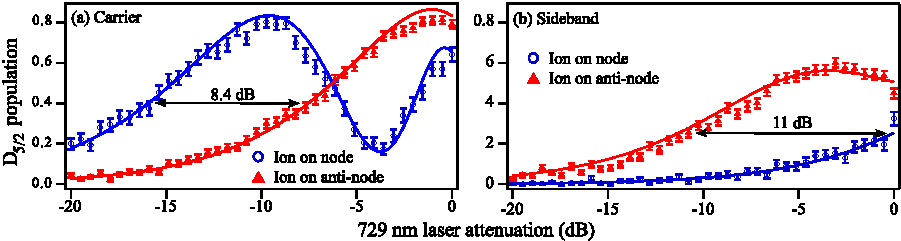
\includegraphics{figures/4/Fig_powerdb}
        \caption{\label{fig:PowerScans} $D_{5/2}$ populations vs. relative laser beam power measured after (a) carrier and (b) red sideband transitions. Interaction time is fixed for both cases (13~$\mu$s). The populations were measured with the ion on either a node (blue circles, $E_y = -0.08$ kV/m) or an adjacent anti-node (red triangles, $E_y = -0.01$ kV/m) near the RF null ($J_0(\kappa) \approx 1$). An effective suppression of 8.4 dB for the carrier and 11 dB for the sideband is achieved. The solid lines represent a simultaneous fit to the data using the model described in the text. For reference, the results from Fig.~\ref{fig:fringes} (a) and (b) were acquired at -13.5 dB and -4 dB, respectively.}
    \end{center}
\end{figure}

In Fig. \ref{fig:PowerScans} we measured $D_{5/2}$ populations after driving the carrier and red sideband transitions as a function of applied laser power. The interaction time was once again fixed (13 $\mu$s, as before). We performed this experiment with the ion on both a standing wave node and antinode, using the results in Fig. \ref{fig:fringes} to select appropriate displacement fields $E_y$. Choosing a node and antinode close to the RF null minimized the micromotion modulation. By measuring the separation between the node and antinode curves, we are able determine the amount of carrier and sideband suppression achieved in our setup. For the carrier, the suppression is equivalent to an 8.4 dB reduction in driving laser power. For the sideband, and equivalent 11 dB reduction can be achieved. 



\subsection{Data fits}

To produce the fits seen in Figs. \ref{fig:fringes} and \ref{fig:PowerScans}, we use Eq. \ref{eq:Pe} to calculate $P_e(t)$ in the case of $\delta = 0$:
\begin{equation}
P_e(t) = \mathlarger{\sum_{n=0}^{\infty}} P_n (\bar{n}) \sin^2 \bigg[ \frac{1}{2} \ J_0(\kappa) \ \Omega_{car/rsb}(\gamma, n) \ t \bigg] \text{,}
\end{equation}
where the coupling strengths are those from Eqs. \ref{eq:OmegaCarSW} or \ref{eq:OmegaSbSW}, respectively. We parameterize a simultaneous fit with 
\begin{equation}
\kappa^2 = \sum_{j=2}^{4} m_j E_y^j
\end{equation}
for the micromotion parameter, and 
\begin{equation}
y = \sum_{j=0}^{4} a_j E_y^j
\end{equation}
for $\gamma = k y \cos \alpha$ , with $m_j$ and $a_j$ the respective fit coefficients. These coefficients, along with $\Omega_1$, $\Omega_2$, $\alpha$, and $\bar{n}$ form the complete set of parameters that defines the simultaneous fits in Figs. \ref{fig:fringes} and \ref{fig:PowerScans}. In particular, we have in this case $|\alpha| = 18^o$, $\Omega_2 / \Omega_1 = 0.52$, and $\bar{n} = 18$. The deviation between the data and the fit near $E_y \approx 0.05$ kV/m in Fig. \ref{fig:fringes} (c) may be due to interactions with light scattered from the trap surface. Otherwise, we see no other significant deviations. The values of $\alpha$ and $\Omega_2 / \Omega_1$ are consistent with the incomplete suppression we measure for the carrier and sideband. 



\subsection{Comparison with numerical models}

Using both the experimental and fitting data we have compared our results to those from a numerical model of our trapping potentials. From the fringe data in Fig. \ref{fig:fringes} we can infer the ion's displacement $y$ as a function of $E_y$ (since fringe maxima corresponds to half a wavelength). From $\kappa^2$ we can determine the pseudopotential $V_{pp}$ as a function of $E_y$ as well. Fig. \ref{fig:model} plots $y(E_y)$ and $V_{pp}(E_y)$ along with their respective predictions from the model. We see good agreement between the respective data sets, providing a measure of confidence in the model for future use. The model includes a 700 V/m uniform stray field that was adjusted to match the observed RF null in Fig. \ref{fig:fringes}. Also. the magnitude of the RF potential in the model was adjusted to match the observed mode frequency at $E_y = 0$. Otherwise, there are no other free parameters used in the model. 

\begin{figure}[htb]
    \begin{center}
        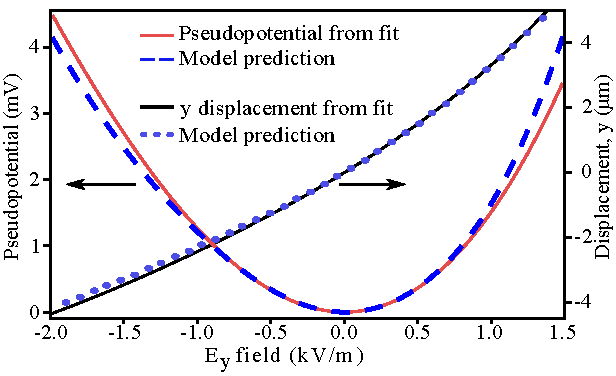
\includegraphics{figures/4/Fig_PPfit}
        \caption{\label{fig:model} Dependence of the pseudopotential $V_{pp}$ and ion displacement $y$ on the applied field $E_y$, along with predictions from a numerical model of the trapping potentials. Deviations from the model can be attributed non-uniformity of the stray fields in the trapping region. }
    \end{center}
\end{figure}




%%%%%%%%%%%%%%%%%%%%%%%%%%%%%%%%
\section{Discussion}

As discussed in Sec. 4.1, the degree of carrier and sideband suppression achievable ultimately depends on the quality of the standing wave field at the ion's position, which, aside from the incident angle $\alpha$, is related to the ratio $\Omega_2\, / \, \Omega_1$. The value $\Omega_2 / \Omega_1 = 0.52$ in our experiment suggests either spacial misalignments in the incident and reflected beams, scattering of the reflected beam from the trap's surface features, or some combination thereof. The Gen IIc trap's surface reflectivity places a limit on $\Omega_2\, / \, \Omega_1=\sqrt{0.86}=0.93$. Approaching this limit would allow for a carrier suppression equivalent to a 29 dB reduction in laser power when $\bar{n}\approx0$ and $|\alpha|<10^{\circ}$. Further carrier suppression would require the use of a different trap with a more reflective surface. For instance, we measure the reflectivity from a gold coated trap like the one described Ref. \cite{Guise15.JAP.117.174901} to be $>98\%$, which could provide an equivalent carrier suppression of $>\,$40 dB. Similar quality standing waves could be generated by incorporating a metallic mirror adjacent to an ion trap--however, phase fluctuations in the standing wave field could become an issue in such a configuration.

Suppression of the carrier implies that the driving laser's power may be freely increased by an amount equivalent to the effective suppression, allowing for faster sideband interactions with no increased chance of an off-resonant carrier excitation. For the 8.4 dB effective carrier suppression we achieve, sideband interactions could be performed 2.5 times faster; at the 29 dB suppression limit of our aluminum trap, 28 times faster; at the $>\,$40 dB suppression limit of a gold coated trap, $>\,$100 times faster.

%%%%%%%%%%%%%%%%
% Chapter 5
%%%%%%%%%%%%%%%%

\chapter{Multi-ensemble atomic clocks with adaptive measurements}

This chapter describes work done towards implementation of multiple atomic ensembles and adaptive measurement techniques in an ion-based atomic clock. These methods were proposed in a paper by J. Borregaard and A. S. S\o rensen \cite{BorregaardSorensen} as a way to improve clock performance when the interrogating local oscillator (LO) is of limited quality. Implementing these methods in a lab-scale  system such as ours is a step towards realizing small-scale frequency references with suitably high performance. 

We will first discuss the basic principles of atomic frequency standards and how they are characterized. We will then review the aforementioned multi-ensemble and adaptive measurement methods proposed in Ref. \cite{BorregaardSorensen}. From there we will discuss the merits of implementing these methods in a $^{40}$Ca$^+$ based clock, and present a scheme for doing so (which is ultimately beyond the scope of this thesis). Finally, we will show preliminary results towards realizing this scheme, and discuss what steps should be taken next to continue this work. 





%%%%%%%%%%%%%%%%%%%%%%%%%%%

\section{Characterization of frequency standards}

An ideal frequency standard is a measurable periodic signal with a stable reference frequency $f_0$. Any signal generated by a real world device will inherently be subject to noise in both the measurement process and in the frequency of the oscillator \cite{RevModPhys.87.637}, resulting in an instantaneous signal frequency $f(t)$ which can waiver from $f_0$. Such a noisy signal can be written as \footnote{We ignore amplitude noise here.}
\begin{equation}  
A(t) = A_0 \sin{(2 \pi f_0 t + \phi (t))}
\end{equation}
where $\phi(t)$ represents fluctuations in the signal's phase away from the nominal phase $2 \pi f_0 t$. Instantaneous frequency drifts in a reference oscillator are generally described by the fractional frequency offset $y(t)$, which is proportional to $\dot{\phi} (t)$ \cite{FreqStands}:
\begin{equation}
y(t) = \frac{f(t) - f_0}{f_0} = \frac{1}{2 \pi f_0} \dot{\phi} (t) \, \text{.}
\label{eq:fracfreq}
\end{equation}
This implies that the average fractional frequency offset over some interval $\tau$ is
\begin{equation}
\bar{y} = \frac{1}{\tau} \int_{t}^{t + \tau}{y (t)} \ dt = \frac{1}{2 \pi f_0 \tau} ( \phi (t + \tau) - \phi (t) ) \ \text{.}
\label{eq:ybar}
\end{equation}
In this way, phase noise and frequency noise in the oscillator are directly related when we are considering the performance of a frequency standard. Measuring one gives us information about the other. 

In the frequency domain, the frequency stability of a reference oscillator is generally characterized by a power spectral density (PSD) function $S_y (f)$ of the function $y (t)$ (for frequencies $f \geq 0$). This function is typically modeled by a power law series which represents five specific noise types in the oscillator \cite{5570702,FreqStands}:
\begin{equation}
S_y (f) = h_{-2} f^{-2} + h_{-1} f^{-1} + h_{0} f^{0} + h_{1} f^{1} + h_{2} f^{2} 
\end{equation}
where $ h_{-2} f^{-2}$ represents random-walk frequency noise,  $h_{-1} f^{-1}$ represents flicker (aka pink) frequency noise, $h_{0} f^{0}$ represents white frequency noise, $h_{1} f^{1}$ represents flicker/pink phase noise, and $h_{2} f^{2}$ represents white phase noise. Fig. \ref{fig:PSDmodel} plots how $S_y (f)$ manifests for the different types of noise described. 

\begin{figure*}[tb]
    \begin{center}
        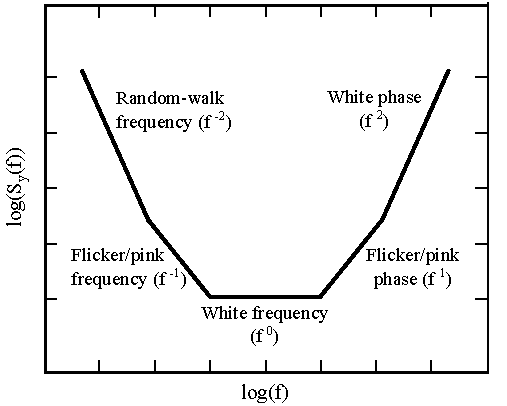
\includegraphics{figures/5/Fig_powerlaw}
        \caption{\label{fig:PSDmodel} Frequency noise power spectral density characteristics of a reference oscillator when modeled with power law series.}
    \end{center}
\end{figure*}

In the time domain, the frequency stability of a reference oscillator is generally derived from a set of successive measurements $\bar{y}_k$ over a common interval length $T$, where each $\bar{y}_k$ value is treated as a random variable. In this case, the standard metric for characterizing the time domain frequency stability of an oscillator is the two-sample Allan variance, defined as \cite{5570702, Allan}
\begin{equation}
\sigma_y^2 (\tau) = \frac{1}{2} \big\langle(\bar{y}_{k+1} - \bar{y}_k)^2 \big\rangle \ \text{.}
\end{equation}
The Allan variance assumes the simplest case of there being no (or negligible) dead time between measurements. It is worth noting that the Allan variance is a sample variance--it is estimated from a finite number two-sample variance values $\frac{1}{2} (y_{k+1} - y_k)^2$ which are averaged to obtain $\sigma_y^2 (T)$.


Atomic frequency standards use the energy splittings between the internal states of an atom, which are proportional to a frequency by Planck's constant, as a stable frequency reference. %For instance, the SI second  is officially defined as ''the duration of 9,192,631,770 periods of the radiation corresponding to the transition between the two hyperfine levels of the ground state of the caesium 133 atom.'' 
A reference atom, or ensemble of atoms, is interrogated by a local oscillator (LO) tuned near to the resonance frequency. The resulting signal from the resonant interaction can be measured and used to produce an error signal, which adjusts the noisy LO's frequency to best match the atomic frequency. This occurs periodically in intervals of $T_c$, such that the LO frequency remains matched to the reference frequency as best as can be accomplished over many intervals.

A common measurement scheme used to interrogate the atomic ensemble and produce the error signal  is the Ramsey method \cite{Rosenband, Ramsey}, which will be described in the next section. When using the Ramsey method, the standard quantum limit for the Allan variance becomes 
\begin{equation}
\sigma_y (\tau) = \sqrt{\sigma_y^2 (\tau)} = \frac{1}{2 \pi f_0 \sqrt{N T \tau}} \ \text{,}
\label{eq:shotlimit}
\end{equation}
where $N$ is the number of independent atoms in the ensemble and $\tau$ is the long-term averaging time \cite{Itano1993}. Beyond the choice of reference frequency $f_0$, the quantum limit in Eq. \ref{eq:shotlimit} is dependent on $N$, as well as the interrogation time $T$. Together these factors determine the limit of achievable performance in an atomic clock. 





%%%%%%%%%%%%%%%%%%%%%%%%%%%

\section{Ramsey interrogations in atomic clocks}

\begin{figure*}[hp]
    \begin{center}
        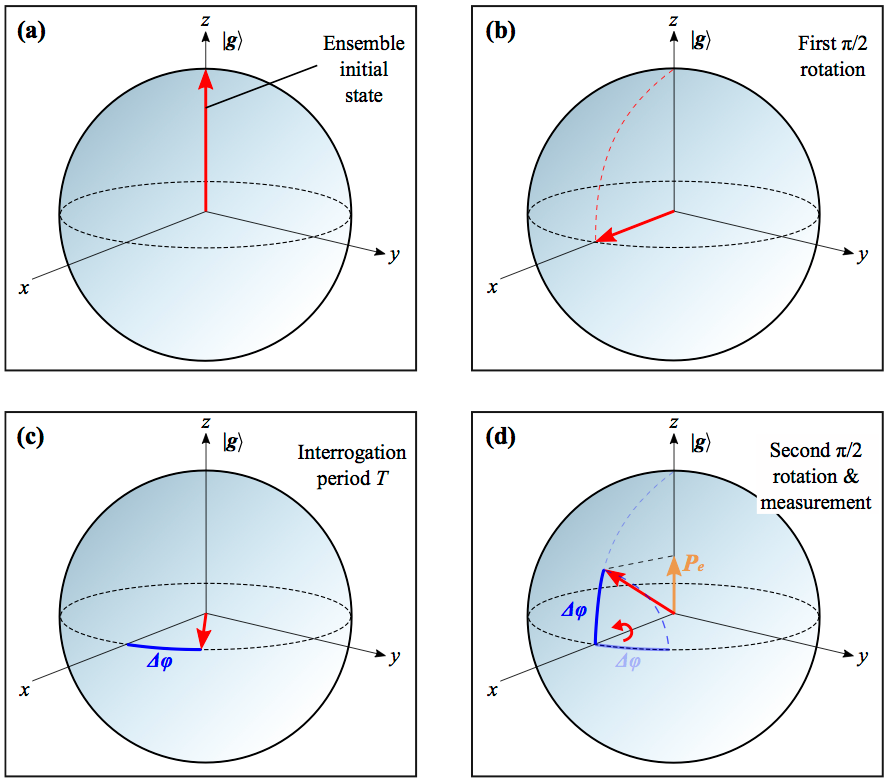
\includegraphics{figures/5/Fig_BlochRamsey2}
        \caption{\label{fig:bloch} Ramsey measurement sequence illustrated in the Bloch sphere representation, which represents the 2-dimension complex Hilbert space in  Eq. \ref{eq:stateEvol}. (a) First, the initial atomic ensemble state (red arrow) is prepared in the ground state $|g \rangle$, corresponding to the z-axis of the Bloch sphere. (b) Second, the state is rotated 90$^{\circ}$ about the y-axis by a $\pi / 2$ pulse from the LO. (c) Third, the state free-evolves for the interrogation time $T$, accumulating phase $\Delta \phi$ from the noise in the LO. (d) Finally, the state is rotated 90$^{\circ}$ about the x-axis by a second $\pi / 2$ pulse, and $P_e$ is measured. Measurement projects the state onto the z-axis and carries an imprint of $\Delta \phi$ which can be used to produce the error signal for the clock. }
    \end{center}
\end{figure*}


Fig. \ref{fig:bloch} illustrates a Ramsey interrogation/measurement sequence in the Bloch sphere representation, which is a convenient visual representation of the 2-dimensional complex Hilbert space defining the time evolution in Eq. \ref{eq:stateEvol}. The measurement works as follows: First, the atomic ensemble to be interrogated is prepared in the ground state $|g\rangle = \begin{psmallmatrix} 1 \\ 0 \end{psmallmatrix}$. The atoms are then excited by the LO radiation at time $t$, for a duration $T_{\pi/2}$ such that $\Omega T_{\pi/2} = \pi / 2$ (where $\Omega$ is the coupling strength, as usual). We refer to these as $\pi/2$ pulses. The first pulse defines the phase between the LO and the atoms and leaves them in the state $\psi_1 = \frac{1}{\sqrt{2}} \begin{psmallmatrix}1 \\ -i \end{psmallmatrix}$, corresponding to a 90$^{\circ}$ rotation about the y-axis of the Bloch sphere\footnote{The axes are arbitrary until the phase between the LO and the atoms is defined by the first pulse.}. The atoms are then allowed to free-evolve for the interrogation period $T \gg T_{\pi/2}$. Any phase difference $\Delta \phi$ which accumulates between the noisy LO and the atoms during this time leaves them in the state $\psi_2 = \begin{psmallmatrix}1 & 0 \\ 0 & e^{-i \Delta \phi} \end{psmallmatrix} \psi_1$. Finally, at time $t + T$ the ensemble is given a second $\pi /2$ pulse, this time with a $\pi / 2$ phase shift in the LO relative to the first pulse. This corresponds to a 90$^{\circ}$ rotation about the x-axis of the Bloch sphere. A state detection is now made on the ensemble, giving
 $P_e(t+T) = N_e / N$ where $N_e$ is number of atoms projected into excited state $|e\rangle = \begin{psmallmatrix}0\\1 \end{psmallmatrix}$.

If $\Delta \phi = 0$ after the interrogation, then $\psi_1$ will have been recovered after the second $\pi / 2$ pulse, and $P_e(t+T) = 0.5$  (assuming perfect measurement). If $\Delta \phi \neq 0$ then the accumulated phase will be imprinted on the resulting measurement of $P_e(t+T)$. The purpose of phase-shifting the second $\pi / 2$ pulse is simply to maximize measurement sensitivity for small $\Delta \phi$.  From $\Delta \phi = \phi (t+T) - \phi (t)$ we may infer $\bar{y}$ for the interrogation interval, as per Eq. \ref{eq:ybar}, and produce the error signal. Any error or noise in the measurement process will also be imprinted on the LO--the probabilistic nature of the state measurement, for instance, leads to the $1/\sqrt{N}$ dependence in the quantum limit (Eq. \ref{eq:shotlimit}). Stochastic sources of error/noise will be averaged down over many cycles of the clock. %, as can be seen in Fig. TBD.


\begin{figure*}[t]
    \begin{center}
        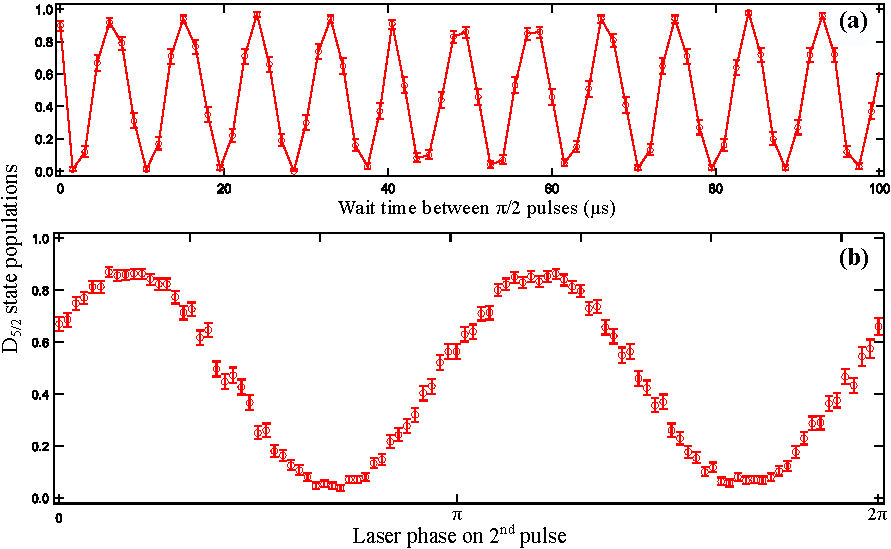
\includegraphics{figures/5/Fig_RamseyEx}
        \caption{\label{fig:RamseyEx} Two examples of Ramsey measurement data. (a) Ramsey measurements with varying interrogation times between the two $\pi / 2$ pulses. In this example, the second pulse was not shifted in phase relative to the first--this merely shifts the phase of the resulting data. The oscillations seen are due to the frequency detuning between the 729 nm laser and the ion (about 4 kHz in this instance). (b) Measurements made with no wait time between the two pulses, but with a varying phase in the second pulse. The purpose of the comparison is to demonstrate how a frequency difference between the LO and ion accumulates over time as a phase difference between the first and second pulses.
           }
    \end{center}
\end{figure*}

The measurement outcomes of a Ramsey sequence will take a $\sin^2$ profile in $\Delta \phi$; Fig. \ref{fig:RamseyEx} shows how this manifests in actual ion measurements. For clock operation, we are restricted to making measurements within the invertible region $|\Delta \phi| \leq \pi/2$. Beyond this range, the periodicity of the sinusoidal signal will result in degenerate measurements of $\bar{y}$, leading to significant over or under-corrections in the LO frequency that will degrade performance.






%%%%%%%%%%%%%%%%%%%%%%%%%%%%%%%%

\section{Improved LO stability with multiple atomic ensembles and adaptive measurements} 


\subsection{Clocks with multiple atomic ensembles}

The performance of an atomic clock is bound by the quantum limit in Eq. \ref{eq:shotlimit}. Because the reference frequency $f_0$ is fixed in a given clock, its best possible performance is dependent on the number of atoms $N$ and the interrogation time $T$. The number of atoms which can be practically implemented is usually limited by systematic factors. For instance, there may be electric field gradients over the spatial extent of large a ensemble cloud, or portions of the cloud which extend beyond the null of the RF trapping field. Uniformly addressing a large cloud with a gaussian optical beam can also be challenging. The interrogation time is limited by the necessity of measuring within the invertible region $|\Delta \phi| \leq \pi/2$. A noisier LO will accumulate phase more rapidly than a less noisy one, and will therefore have a more limited interrogation time. As such, the quality of the LO limits the long-term stability of a clock.

\begin{figure*}[ht]
   \begin{center}
        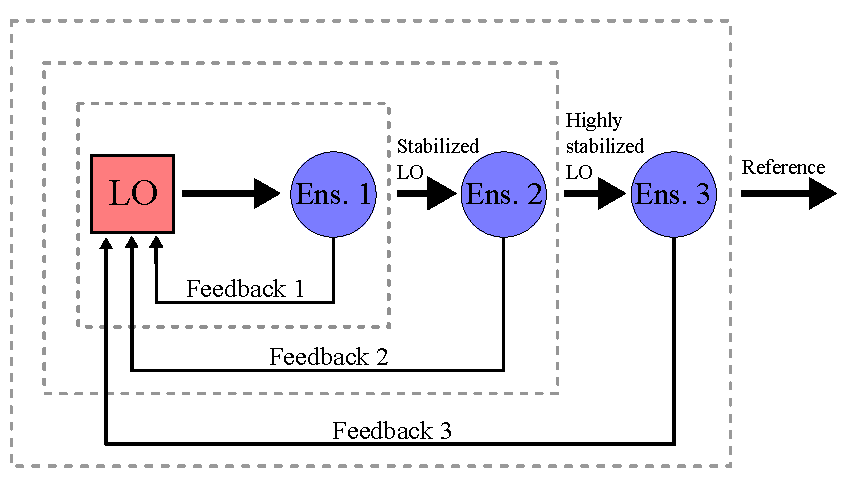
\includegraphics{figures/5/Fig_multiensembles}
        \caption{\label{fig:multiensemble} Illustration of locking the LO using multiple ensembles ($m = 3$, in this case). The first ensemble is interrogated for a time $T_1$ during the interrogation of the second and third ensembles. $T_1$ is sufficiently limited to keep the measurement within the invertible region $|\Delta \phi| \leq \pi/2$. Feedback from the first ensemble stabilizes the LO such that the second ensemble can be interrogated for $T_2 > T_1$. Feedback from the second ensemble further stabilizes the LO allows for $T_3 > T_2$, and so on. This method improves the stability of the clock by $N^{-(m/2)}$, where $m$ is the number of ensembles containing $N$ atoms each. }
    \end{center}
\end{figure*}


A proposal by Borregaard and S\o{}rensen \cite{BorregaardSorensen} describes novel methods by which interrogation times may be improved. First, they show that by locking the LO to several atomic ensembles instead of one, an improvement in stability (i.e. a decrease in $\sigma_y(\tau)$ in Eq. \ref{eq:shotlimit}) can be achieved which is proportional to $N^{-(m/2)}$, where $m$ is the number of ensembles containing $N$ atoms each. Fig. \ref{fig:multiensemble} illustrates how this method works. In essence, a single ensemble has a limited interrogation time $T_{1,max}$ due to the need to keep $\Delta \phi$ within the invertible region. If a second ensemble is interrogated simultaneously with $T_2 > T_{1,max}$, and the feedback from the first ensemble is used to correct the LO at some time $T_{1,max} < t < T_2$, then the $T_2$ interrogation of the second ensemble will not exceed the invertible region (within some limit $T_{2,max}$). The resulting correction from the second ensemble will provide a greater LO stabilization than would be achieved with regular measurement techniques. Adding subsequent ensembles to this feedback chain increases the resulting LO stability. For $m$ ensembles of $N$ ions each, the stability of the clock is, expressly,
\begin{equation}
\sigma_y (\tau) = \frac{1}{2 \pi f_0 \sqrt{\tau} } \frac{1}{(N \gamma \ T_{1,max})^{(m/2)}}  \sqrt{\gamma \ (\beta_1 / \beta)^{(m-1)} }
\label{eq:clockstab}
\end{equation}    
where $\gamma$ is a parameter characterizing the LO noise, and $\beta_1$ and $\beta$ are constants dependent on the noise spectrum of the uncorrected and corrected LO, respectively \cite{BorregaardSorensen}. Note that when $m = 1$, Eq. \ref{eq:shotlimit} is recovered.  


In Eq. \ref{eq:clockstab} we see that the clock stability is still limited by the maximum interrogation time of a single ensemble $T_{1,max}$, as well as the number of atoms per ensemble $N$. Simulations show that $\gamma T_{1,max} = 0.1$ is a limit above which improvement in the clock stability begins to be lost \cite{BorregaardSorensen}. For this upper value of $T_{1,max}$, ``break even'' improvement is achievable for as few as $N = 20$ atoms per ensemble in this protocol. Any fewer, and the resulting quantum projection noise from the first measurement injects too much noise into the second, such that the improvement becomes less than what would be achieved by simply having a single ensemble of $m N$ atoms. For $N_{min} = 20$, a factor of $\sim \sqrt{2^{(m-1)} }$ improvement in stability is predicted. 

%%%% 

\subsection{Adaptive measurement techniques in clock interrogations}


\begin{figure*}[ht]
    \begin{center}
        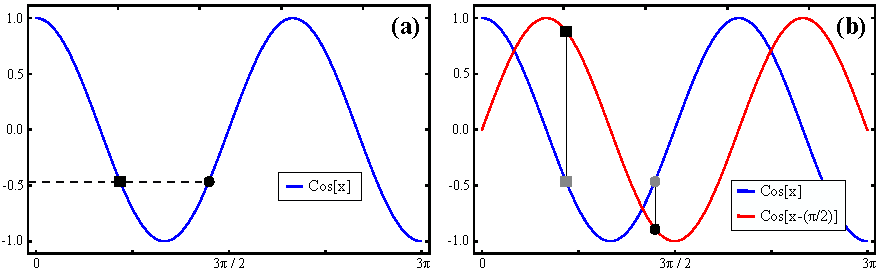
\includegraphics{figures/5/Fig_quadrature}
        \caption{\label{fig:quadrature} (a) Two points (circle, square) on a sinusoidal phase (blue curve) that are indistinguishable when measured. This limits the effective measurement range to $\pm \pi / 2$ at maximum, hence the invertible region restriction in Ramsey measurements. (b) The same two points measured with a phase shift of $\pi / 2$ (red curve). The addition of this phase shifted measurement distinguishes the two points and extends the measurement range to $\pm \pi$. This is also called a quadrature measurement. }
    \end{center}
\end{figure*}

To improve performance even further, the authors introduce an ``adaptive'' measurement technique \cite{BSsup}. In this method, Ramsey measurements of an ensemble are initiated as normal (a single $\pi / 2$ pulse on all atoms), but completed sequentially on subsets of the ensemble rather that on all atoms simultaneously. After a subset measurement, during which the remainder of the ensemble is still being interrogated, an intermittent adjustment can be made to the phase of the LO (not the frequency) before measuring the next subset. The subsequent measurement's outcome is therefore correlated to the first in a way which extends the invertible region beyond $\pm \pi / 2$ to $\pm \pi$, assuming that the measurements occur on a timescale $\ll T_{max}$. In principle this is similar to making a quadrature measurement, in which sampling a sinusoidal signal at both 0 and $\pi / 2$ phase offsets gives more information (Fig. \ref{fig:quadrature} (b)). The adaptive measurement method, however, involves a Bayesian analysis after each subset measurement in order to predict the LO phase shift which will maximize the sensitivity of the following measurement. 

The net result is to increase the invertible region of the error signal, and consequently increase $T_{1,max}$, for the ensemble as a whole. Specifically, the limit of $\gamma T_{1,max}$ is relaxed from 0.1 to (up to) 0.3. Subsequently, Eq. \ref{eq:clockstab} predicts $N_{min} = 4 \ (7)$ when using this protocol in the case of white ($1/f$) LO noise. 

%\begin{figure*}[t]
 %   \begin{center}
 %       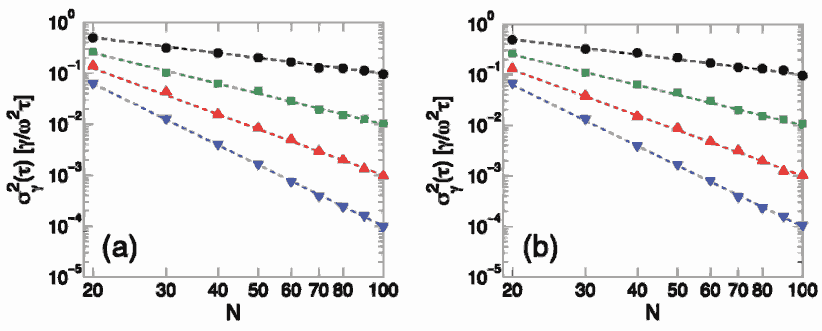
\includegraphics{figures/5/Fig3}
    %    \caption{\label{fig:adaptsim} Figures from Ref. \cite{BorregaardSorensen}. Simulated Allan variance measurements for a system of 1, 2, 3, and 4 ensembles (black, green, red, blue) of N ions. White LO noise is simulated. The simulations measure $\sigma_y^2 ({\tau})$ in the cases of (a) standard Ramsey measurements and (b) the adaptive measurements described in \cite{BSsup}.     }
   % \end{center}
%\end{figure*}








%%%%%%%%%%%%%%%%%%%%%%%%

\section{Implementation in a $^{40}$Ca$^+$ optical clock}

Our primary long-term goal in this project is to improve LO performance in a trapped ion clock by implementing multi-ensemble and adaptive measurement techniques. We believe that such a clock will be an excellent candidate for the basis of small-scale, portable frequency references. Decreased LO quality is one of the primary technical hurdles in building a high performance small-scale device, particularly one based on an optical reference frequency as lasers are usually stabilized to large, heavy glass cavities. A clock based on our $^{40}$Ca$^+$ system already has several advantages when considering adaptations to small-scale device: First, choosing the suitably narrow $S_{1/2} \leftrightarrow D_{5/2}$ transition as the reference means that the interrogating LO will be the 729 nm laser, which is in the optical frequency range ($f_0 \sim 10^{14}$ Hz). The $1/f_0$ dependence in Eq. \ref{eq:shotlimit} gives optical clocks\footnote{A good overview of optical clocks is provided in Ref. \cite{OpticalClocks}.} a natural advantage in stability over microwave frequency clocks such as caesium standards, which have $f_0 \sim 10^9 - 10^{10}$ Hz. Despite there being probeable atomic transitions with substantially greater frequencies than those in the optical range, such as M\"{o}ssbauer transitions on the order of $10^{19}$ Hz \cite{OpticalClocks}, LOs in the optical range meet the requirements of 1) being producible with a sufficiently narrow linewidth, due to the development of lasers and cavity-based stabilization \cite{StableLaser1, 6174186,McFerran:12,KesslerT.2012,Y.2011,PhysRevA.79.053829,Dubé2009,Ludlow:07, PhysRevLett.82.3799} and 2) having countable cycles, due to the development of optical frequency combs \cite{R.2008,RevModPhys.78.1297,Grosche2008,RevModPhys.78.1279,RevModPhys.75.325,Udem:99, PhysRevLett.88.073601,PhysRevLett.84.5102}. A particular advantage to using $^{40}$Ca$^+$  is that many other ion species only have suitable optical transitions in the UV range, which are not as easily producible. Second, planar ion traps like the one used in this work already have demonstrated scalability (the Gen IIc for instance is already on the order of 1 cm$^2$). Third, although fewer atoms will participate in the clock measurement than in thermal vapor or optical lattice based devices, a clock based on trapped/cooled ions have longer coherence times (see next section) and will therefore allow longer interrogation times, increasing the overall sensitivity per atom/ion. 

For realizing a multi-ensemble clock, we must be able to load and confine multiple ions. This is already within the capabilities of our Gen IIc trap, which has previously demonstrated a single linear chain of 10 ions \cite{IonTrap}. A similar GTRI planar trap in our lab has recently loaded 35 ions in a single linear chain, so there is room yet for improvement in our system. The ability to separate chains into multiple ensembles or subsets of ensembles is inherent to the design of our traps and is used for deterministic loading and to perform quantum gates \cite{Kielpinski2002}. 

For performing adaptive measurements, we must be able to interrogate and measure individual ions or subsets in an ensemble. There are several options available to us in our system, each with different merits. First, our use of an optical frequency LO and state-detection beam makes single-ion addressing possible, since focused beam waists can be realized that are several times less than the typical ion spacing in a linear chain ($\sim$ 3-7 $\mu$m). Precision beam-steering can be technically challenging to implement, however. An alternative to single-ion addressing involves separating a subset of ions from a larger chain and transporting them to a location where they can be independently interrogated/measured. This requires that transport operation be performed within the timescale of both the overall interrogation time and the state coherence time of the ions. Finally, arbitrary state rotations can also be achieved by dynamically transporting an ion through a static, steady-state beam \cite{TransGateTh,TransGateExp}. Because high-speed beam pulsing typically requires the use of AOMs and their peripheral hardware, this so-called transport method of state control is advantageous in that it does not require this additional hardware overhead. However, achieving the precise transport necessary for this method can be technically challenging. 




%%%%%%%%%%%%%%%%%%%%%%%%%%%%

\section{Research goals}


%%%%%%%%%%%%%%


\begin{figure*}[hp]
    \begin{center}
        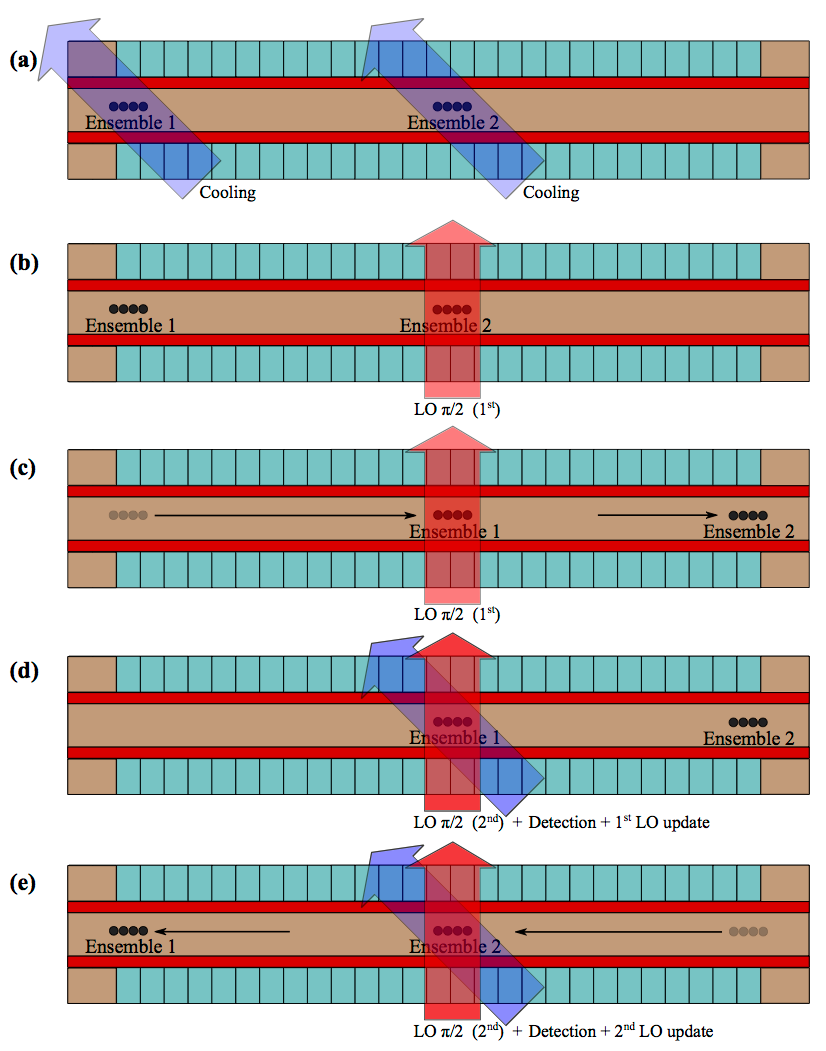
\includegraphics{figures/5/Fig_ClockScheme3}
        \caption{\label{fig:clockscheme} A possible scheme for a 2-ensemble clock in our system. (a) Ensembles 1 and 2 are initialized and cooled. (b) Ensemble 2 receives the first $\pi / 2$ pulse of a Ramsey measurement. (c) Ensemble 2 is transported away and begins its interrogation period; Ensemble 1 is transported in, receives its first $\pi / 2$ pulse, and free-evolves for $T_1 \leq T_{1,max}$. (d) Ensemble 2 continues to free-evolve; Ensemble 1 receives its second $\pi / 2$ pulse, followed by a state detection and update to the LO frequency. (e) Ensemble 1 is transported back to its beginning point; Ensemble 2 completes its interrogation period $T_2 \leq T_{2,max}$ and is transported back to its start point. A final $\pi /2$ pulse and state detection occurs, and the LO is updated again. The entire cycle now repeats. Adding adaptive measurements simply involves intermittent steps after (c) to divide the ensembles into appropriate subsets.   }
    \end{center}
\end{figure*}

Fig. \ref{fig:clockscheme} shows a potential scheme for how a 2-ensemble clock with adaptive measurements could be realized in our $^{40}$Ca$^+$ system. This scheme uses ion/subset transport for interrogating/measuring multiple ensembles. Successful implementation will have several key technical requirements: first, we must show that ion coherence times in our system are not prohibitively short, both for single ions and for ensembles. Decoherence refers to the degradation of an ion's superposition state over time, due to coupling of the Hamiltonian to the external environment \cite{PhysRevA.57.3748, SACKETT2003431, RevModPhys.75.715}. Because Ramsey interrogations occur while ions are in a superposition state of the reference transition, decoherence will limit achievable interrogation times. Although we have previously measured single-ion coherence times of $\sim$ 1-1.5 ms in our system, which is generally sufficient for basic clock operation, the scheme in Fig. \ref{fig:clockscheme} includes transport operations which must be performed on a similar timescale. The current stabilization cavity for the 729 nm laser should allow for 10-100 ms coherence times if all other factors are accounted for. Second, we must characterize and minimize ``state destruction'' events which occur when Ramsey superposition states experience unwanted interactions with the 397 nm laser. This can happen when scattered (or edge-of-beam) light from a state detection event reaches an ion in the middle of a Ramsey interrogation elsewhere (see Fig. \ref{fig:clockscheme} (d), for instance). 

Beyond these primary requirements, realization of our proposed scheme will include several key milestones: 1) characterizing systematic factors in our system which could cause frequency shifts in a clock (magnetic field noise, for instance), 2) configuring the our system to function as a simple frequency reference for the 729 nm laser, 3) configuring the system to load, merge, and separate multi-ion ensembles, 4) demonstrating coherent transport of whole ensembles, and 5) performing rapid phase updates to the 729 nm LO during adaptive measurements. Once we have successfully implemented this scheme with a pulsed interrogation beam, we can consider implementing the transport method for ion interrogations instead. 












%%%%%%%%%%%%%%%%%%%%%%%%%%%%%%%%%%%%%%%%%%%%%%%%%

\section{Preliminary results}

In this section we will discuss and show results from preliminary efforts towards realizing a 2-ensemble clock with adaptive measurements in our system. Our focus has been primarily to characterize the key technical aspects of ion decoherence, transport, and state destruction. 

%\subsection{Characterization of systematic frequency shifts}



\subsection{Coherence times of a single ion}

\begin{figure*}[t]
    \begin{center}
        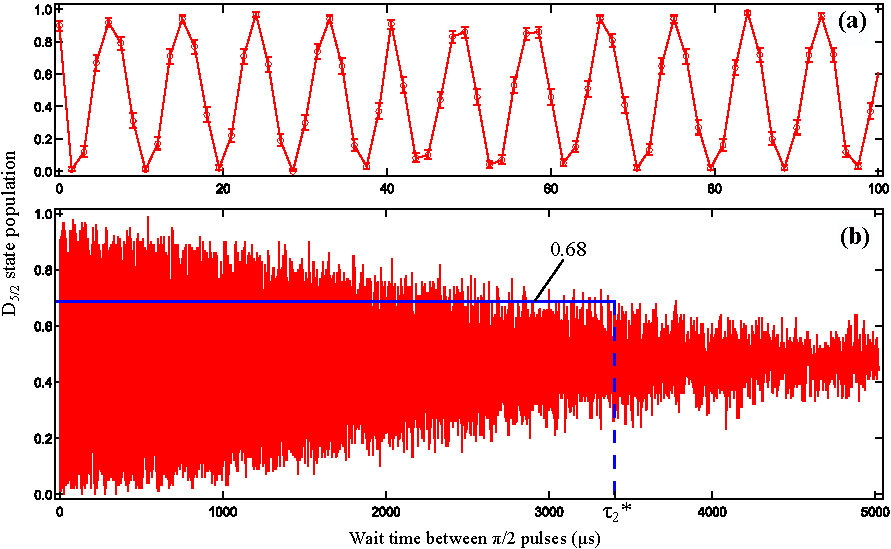
\includegraphics{figures/5/Fig_CoherenceTime2}
        \caption{\label{fig:coherencetime} $D_{5/2}$ populations measured after 2 separate $\pi / 2$ pulses, with a varying wait time between them. Both pulses have the same relative phase set by the laser. (a) The population measurements oscillate at twice the detuning frequency between the ion and the 729 nm laser (about 4 kHz here). (b) The same data over a broader time scale. The overall amplitude of these oscillations decays in time due to decoherence of the ion's superposition state. The coherence time $\tau_2^*$ is defined as the point when the envelope amplitude decays to $\approx 0.68$ (blue line).   }
    \end{center}
\end{figure*}

To measure the coherence time of a single sideband cooled ion ($\bar{n} \approx 0.2$), we perform 2 separate $\pi / 2$ pulses on the $S_{1/2} \rightarrow D_{5/2}$ transition, varying the wait time between them, and measure $P_e$ after the second pulse. The second pulse has the same relative phase as the first, such that $P_e (2 T_{\pi /2}) \approx 1$ when no wait time is applied. The measured $P_e$ values will take a $\sin^2$ profile as they oscillate at twice the detuning frequency between the ion and the laser (just as in a clock interrogation). Decoherence will manifest as an exponential decay in the amplitude of the oscillations over time \cite{PhysRevA.57.3748, SACKETT2003431, RevModPhys.75.715}. The characteristic coherence time $\tau_2^*$ is given by 
\begin{equation}
P_{e,max} (\tau_2^*) = \frac{1}{2} \bigg(1 + \frac{1}{e} \bigg) \approx 0.68
\end{equation}
Fig. \ref{fig:coherencetime} shows a coherence time $\tau_2^* \approx 3.4$ ms measured on the $|S_{1/2}, m_J = 1/2 \rangle \rightarrow |D_{5/2}, m_J = 1/2 \rangle$ transition in our system. In the absence of other systemic factors, we would expect to see coherence times of $\tau_2^* \sim 10-100$ set by the limit of the cavity-stabilized 729 nm linewidth of 10-100 Hz. We believe that we are limited here by either non-ideal gain settings and/or noise in the PID feedback loop \cite{doi:10.1119/1.1286663} of the cavity lock, or by phase-noise modulations introduced to the laser in a 25 m fiber optic cable, due to background mechanical/thermal stressors on the fiber \cite{Ma:94} (or some combination of the two effects). Our belief is based on 1) observed minute-to-minute sensitivity of the coherence time to the quality of the cavity locking feedback signal, 2) observing significant sensitivity in the polarization of fiber-transmitted light when the fibers are squeezed or bent, arising from phase shifts of the light in the medium, and 3) achieving transition linewidths of several hundred Hz at best, consistent with a coherence time of several milliseconds and indicative of either imperfect cavity locking or spectral broadening along the optical pathway. 

\begin{figure*}[ht]
    \begin{center}
        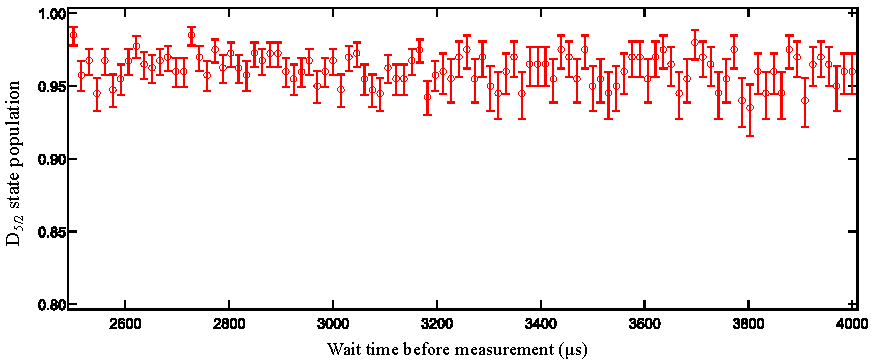
\includegraphics{figures/5/Fig_PopDecay}
        \caption{\label{fig:popflop} $D_{5/2}$ populations measured after a single inverting pulse, followed by a varying wait time. At wait times on the scale of the coherence time $\tau_2^* \approx 3.4 ms$, no significant decay in population is observed, indicating that the steady-state 866 nm laser is not causing unwanted off-resonant transitions on the 854 nm $D_{5/2} \rightarrow P_{3/2}$ transition.    }
    \end{center}
\end{figure*}

We can rule out certain other potential limiting factors in our coherence time: first, we have repeated the measurement on the $|S_{1/2}, m_J = 1/2 \rangle \rightarrow |D_{5/2}, m_J = 5/2 \rangle$ transition, which is 5 times as magnetically sensitive. We did this both with and without 60 Hz triggering of the experiments. In each case, there was no measurable difference on the coherence time, indicating that magnetic field noise effects are relatively negligible. Second, we have repeated the measurement both with and without a 1.5 ms delay added before the first $\pi / 2$ pulse. The pre-delay allows the ion undergo additional heating, on the order of that which would occur in a typical coherence time experiment. In each case, again, there was no measurable difference on the coherence time, indicating that the decay of the superposition state is not due to thermal state dephasing arising from excessive heating. Third, we have tested whether the 866 nm laser, which is continuously steady-state, was potentially causing off-resonant excitations on the 854 nm $D_{5/2} \rightarrow P_{3/2}$ transition. We did this by inverting the population to $P_e \approx 1$ in a single pulse and then measuring after a varying wait time (Fig. \ref{fig:popflop}). No decay in population over time was observed, indicating that potential off-resonant excitations are negligible if not non-existent. 



% Get that decoherence time figure in here

\subsection{Transport heating}

As described in Ch. 3, ion transport in our system is done through incremental updates to the trap's DC electrodes in order to move a harmonic well along the trap axis from point A to B. The granularity of this process will affect an ion's motional state if the transport is done in too few steps. Because our system updates electrode voltages at a rate of 10 kHz, a transport operation performed in $n$ steps will take $n \times 0.1$ ms to complete. To transport an ion within the measured coherence time of $\approx$ 3 ms, we will therefore have to limit the number of steps to $n < 30$. For a transport distance of several hundred $\mu$m or greater, this imparts a significant amount of motion to an ion in our current configuration. Beginning with $\bar{n} \approx 0.2$ sideband cooled ions, we attempted to transport ions over such distances in 15-20 steps, and measure $\bar{n}$ afterwards per Eq. \ref{eq:nbar}. However, we observed population inversions on the red sidebands begin exceed those on the blue sidebands, indicating ions that were no longer in a thermal state described by Eq. \ref{eq:Pn} and therefore rendering Eq. \ref{eq:nbar} invalid. By comparison, adiabatic transports with approximately 1 step per several $\mu$m of travel exhibit no heating beyond that of the trap's inherent heating rate. %Fig. TBD. 
% Refs about reducing heating? Ask True



\subsection{State destruction characterization}

% Branching ratio figure
State destruction occurs when an ion experiences an unwanted interaction with resonant 397 nm light during the middle of a Ramsey interrogation. To characterize state destruction, we must first understand how the resulting state measurement will have been affected. After the first $\pi /2$ pulse but before the second, the ion has an effectively equal chance of being projected into the $D_{5/2}$ or $S_{1/2}$ states by the 397 nm light. When projected into $D_{5/2}$, the second $\pi /2$ pulse of the Ramsey sequence will leave the ion back in the superposition state such that $P_e = 0.5$ on average upon measurement. This particular outcome occurs 50\% of the time on average. When projected into $S_{1/2}$, the ion will subsequently be excited on the $S_{1/2} \rightarrow P_{1/2}$ transition and then decay, with equal probability, to either the $|S_{1/2}, m_J = -1/2 \rangle$ or $|S_{1/2}, m_J = 1/2 \rangle$ ground states. Because the 729 nm LO will be tuned to excite only one of these states, the second $\pi /2$ pulse will either 1) also lead to $P_e = 0.5$ upon measurement (on average), or 2) leave the ion in the ground state, such that $P_e = 0$. Each of these respective outcomes occurs 25\% of the time on average. 


\begin{figure*}[t]
    \begin{center}
        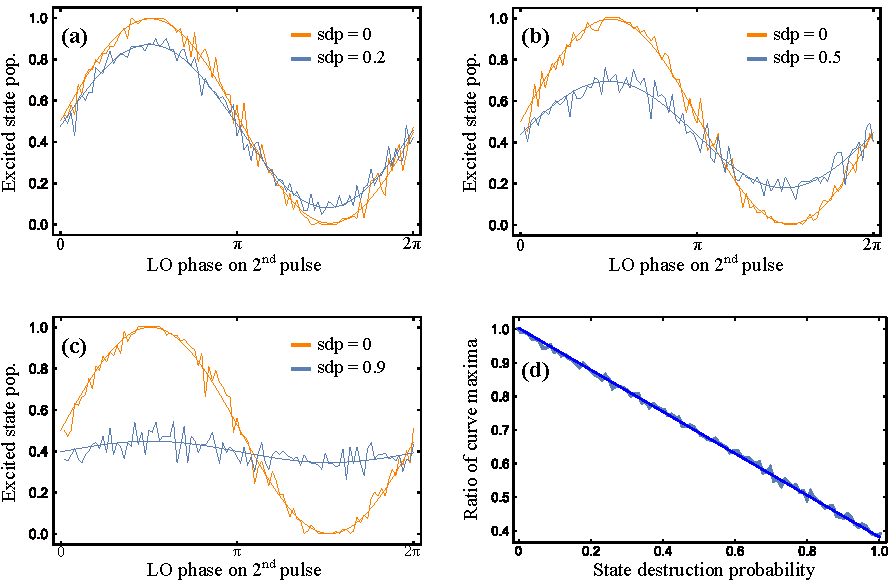
\includegraphics{figures/5/Fig_sdpsims}
        \caption{\label{fig:sdpsim} (a,b,c) Simulated Ramsey measurements with a varying phase on the second $\pi / 2$ pulse, and with state destruction probabilities of (a) 0.2, (b) 0.5, and (c) 0.9 (light blue curves). The $sdp = 0$ case is also plotted in each instance (orange curves). Each point represents the average of 100 measurement sequences (or, equivalently, 1 measurement sequence on 100 atoms). (d) The ratios of the $sdp \neq 0$ maxima to the $sdp = 0$ maxima are effectively linear in $sdp$. }. 
    \end{center}
\end{figure*}

Therefore, in the event of an unwanted interaction with 397 nm light, which we refer to as a state destruction event, the measurement outcome of the Ramsey sequence will be (on average) either $P_e = 0$ or $P_e = 0.5$, with probabilities $1/4$ and $3/4$, respectively. With this knowledge, state destruction can be numerically modeled as a probabilistic event. We consider a Ramsey measurement sequence with two resonant $\pi /2$ pulses, in which the second pulse has a varying relative phase from 0 to $2 \pi$ (as in the measurement in Fig. \ref{fig:RamseyEx} (b)). When no state destruction occurs, the measurement outcomes are probabilistic, with the excited state probability $P_e$ taking a $\sin^2$ profile as a function of the varying phase. When state destruction does occur, the measurement outcome will be $0$ or $0.5$ with probabilities $1/4$ and $3/4$, respectively. We introduce a state destruction probability parameter $sdp$ which determines the likelihood of a state destruction event taking place. Fig. \ref{fig:sdpsim} (a,b,c) shows that by varying $sdp$ from 0 to 1 in the simulation and averaging over a suitable number of measurements, the $\sin^2$ output of the Ramsey sequence gradually decays in amplitude. Each point in the data represents the average of 100 measurement sequences (or, equivalently, 1 measurement sequence on 100 atoms).

The maxima of these sinusoids relative to the $sdp = 0$ case are unique. In Fig. \ref{fig:sdpsim} (d) we measure this ratio for $0 \leq sdp \leq 1$ in increments of 0.1, and find a linear relationship. By parameterizing this relationship, we can perform these same Ramsey sequences in our experiment and quantify state destruction. Specifically, we pulse the 397 nm beam at varying distances from an ion that is between $\pi / 2$ pulses in the sequence described above, then repeat the exact same sequence with no pulse (hence $sdp = 0$ in the no-pulse instance). Fig. \ref{fig:sdp} shows these results. The pulse duration was 200 $\mu$s, which is equivalent to that of a state detection pulse in our system. The total interrogation time was just long enough to allow for the pulse to occur, minimizing decoherence. The 729 nm beam remained at a fixed position throughout ($z = 1000$ on the trap axis). 

\begin{figure*}[t]
    \begin{center}
        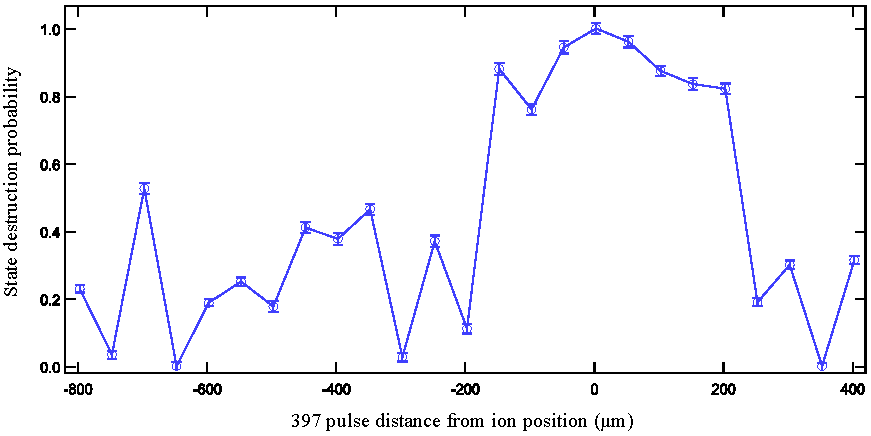
\includegraphics{figures/5/Fig_sdp}
        \caption{\label{fig:sdp} Measured state destruction probabilities in our trap vs. distance of the 397 nm beam from the ion's position ($z = 1000$). }
    \end{center}
\end{figure*}


We estimate the focused 397 nm beam waist to be 40-60 $\mu$m at the trap axis. We see in Fig. \ref{fig:sdp} that state destruction is significant within $\pm 150 \ \mu$m of the ion position, either due to significant nearby scatter from the trap surface or due to interactions with the edge of the beam profile. Beyond this range $sdp$ varies as the light scatters from the different regions of the trap, but for the most part is non-trivial throughout the range of measurement. 







%%%%%%%%%%%%%%%%%%%%%%%%
\section{Discussion}


In order to continue making progress towards a multi-ensemble clock with adaptive measurements, we will need to address these technical limitations discovered thus far. First, we will need to improve on the current single ion coherence time of $\approx$ 3 ms in order to allow for suitably adiabatic transport operations. Improvements to the laser's cavity stabilization can be made through precise calibrations of the PID loop's gain settings, as well as from performing a systematic analysis of any noise which may exist in the feedback signal. Previous experiments in our lab have not required coherence times longer than what we have measured, so it likely that improvements can be made to the cavity lock which were previously unnecessary. Output linewidths approaching 10 Hz should be possible in this cavity, given its finesse. Phase-noise modulation of the laser due to stress on the optical fiber(s) can be reduced by implementing a method demonstrated in Ref. \cite{Ma:94}, in which a portion of the transmitted light is reflected back through the fiber and measured against the input light, allowing the phase difference to be monitored and continuously corrected during experiments. Using this method, the authors reduce the linewidth of 532 nm light transmitted through a 25 m optical fiber from 1.2 kHz to 16 Hz, with only a marginal reduction in carrier power. Assuming no other contributing factors, a similar reduction in linewidth in our system would achieve 50-100 ms coherence times, which should be suitable for adiabatic transport during clock cycles.

Beyond extending the single-ion coherence time, we will need to measure the coherence times for multi-ion ensembles and ensure that they are also suitable for transport. Upgrading the system's digital-to-analog converters would also increase the electrode update rate of 10 kHz and allow for faster transport operations. In Ref. \cite{PhysRevLett.109.080502}, converters with an update rate of 50 MHz were used to diabatically transport single ions and separate two-ion chains on timescales of 10-50 $\mu$s, with overall heating $<$ 2-3 quanta. 

In order to address and reduce state destruction in our system, there are several improvements which can be made easily and immediately. The first would be to reduce the focused waist of the 397 nm detection beam, which will reduce light scatter. A waist of 10-15 $\mu$m is easily achievable for this wavelength with appropriate optics, and would still allow for simultaneous addressing of 4-6 ions in an ensemble. The second would be to better isolate the PMT from ambient room light, which will increase detection efficiencies and allow us to use shorter detection pulses, further reducing the chances of state destruction events. Detection efficiencies of 99.99\% have been demonstrated for both single $^{40}$Ca$^+$ ions and ensembles of 4 \cite{PhysRevLett.100.200502, PhysRevA.81.040302}.  Once these improvements are made, the experiment in Fig. \ref{fig:sdp} can be repeated in the updated configuration, with greater spatial resolution and with varying placements of the 729 nm beam. Thorough knowledge of the state destruction probabilities which occur for the different beam placements will allow us to choose the best ensemble and beam positions in Fig. \ref{fig:clockscheme}. 

% \textit{Blab about simulations?} Even if state destruction cannot be eliminated entirely during ensemble interrogations












%%%%%%%%%%%%%%%%
% Chapter 6
%%%%%%%%%%%%%%%%

\chapter{Conclusion and future outlook}


\section{On motional state control via standing wave beams}

In Ch. 4, we have shown how the coupling strengths of carrier and first order sideband transitions in a trapped ion may be selectively controlled by displacing the ion within a resonant standing wave field. Using the surface of our Gen IIc ion trap as a mirror, we produced a standing wave field at the ion position by reflecting a 729 nm laser off the trap surface, thus avoiding the challenges of in-vacuum optical cavities. As predicted, the carrier and sideband coupling strengths demonstrate a periodic dependence on the ion's position within the standing wave fringes, with the cycles of the two cases 180$^{\circ}$ out of phase with each other. Despite having an imperfect standing wave due to an 18$^{\circ}$ angle in the incident beam and a limited reflectivity from the aluminum trap surface, we were able to achieve equivalent carrier and sideband suppressions of 8.4 dB and 11 dB, respectively. We calculate that a 29 dB equivalent carrier suppression is possible in our configuration with improved beam alignment, whereas in a gold coated trap this figure could be increased to $>$ 40 dB. Recently, we have become aware of a planar ion trap fabricated directly on top of a highly reflective (HR) UV mirror for the specific purpose of achieving a configuration similar to ours \cite{doi:10.1063/1.4970542}. Although the authors do not provide a number, it is reasonable to speculate that such an optimized material could be even more reflective than the gold trap, and could achieve even greater coupling strength suppressions.

Based on our results, we believe that our standing wave configuration is a viable alternative to in-vacuum cavities, and can be advantageous for various experiments in quantum computation and simulation. There are several potential applications of which we are already aware: first, suppression of the carrier allows the driving laser's power to be freely increased by an equivalent amount, allowing for faster sideband interactions with no increased chance of an off-resonant carrier excitation. Such increased speeds could be particularly beneficial in ion trap quantum computations, as they can increase the fidelity of two-qubit gate operations. For the 8.4 dB effective carrier suppression we achieve, sideband interactions could be performed 2.5 times faster; at the 29 dB suppression limit of our aluminum trap, 28 times faster; at the $>\,$40 dB suppression limit of a gold coated trap, $>\,$100 times faster. Second, a 29 dB equivalent carrier suppression factor achievable in our current configuration would reach the regime in which simulating the expansion of the universe with trapped ions becomes experimentally feasible. Per Ref. \cite{Menicucci10.NJP.12.095019}, suppressing the carrier allows for the excitation of detectors due to the creation of cosmic photons. When the beam has more running wave character, the simulation is dominated by excitation of detectors with photon creation or destruction. Third, standing wave configurations such as the one described here have also been considered for quantum phase transition experiments \cite{PhysRevLett.118.073001}.

%Suppression of the carrier implies that the driving laser's power may be freely increased by an amount equivalent to the effective suppression, allowing for faster sideband interactions with no increased chance of an off-resonant carrier excitation. For the 8.4 dB suppression we have achieved, sideband interactions could be performed 2.5 times faster; at the 29 dB suppression limit of our aluminum Gen IIc trap, 28 times faster; at the $>$ 40 dB suppression limit of a gold coated trap, $>$ 100 times faster. Performing faster sideband interactions could, in particular, improve two-qubit gate fidelities in ion trap quantum computers. 




\section{On the implementation of multiple ensembles and adaptive measurements in atomic clocks}

In Ch. 5, we have discussed the merits of multiple ensembles and adaptive measurement techniques in atomic clocks, per a proposal by Borregaard and S\o rensen \cite{BorregaardSorensen}, and have put forth a scheme for implementing these methods in a $^{40}$Ca$^+$ based clock. If successful, these methods would allow for improved clock performance when the local oscillator (LO) is of limited quality, as will inevitably be the case in a small-scale device. Realizing these methods in a laboratory scale experiment would be the first step towards adapting them for small-scale frequency standards, which are in high demand for applications such as GPS and local network synchronization. As we have discussed, we believe that $^{40}$Ca$^+$ based clocks haave unique advantages which make them a good candidate for small-scale integrated devices.   

In preliminary work towards realizing this proposed clock scheme, we have measured a single-ion coherence time of $\tau_2^* \approx 3.4$ ms in our system. Our scheme includes several ion transport operations which must be performed adiabatically, and the update rate of our trap electrodes limits these steps to durations of several ms at the least. As such, this coherence time is prohibitively short for our needs. However, our results suggest that the coherence time is limited by the linewidth of the 729 nm laser at the ion, due to either noise/imperfections in the cavity stabilization feedback loop, or to phase noise modulation occurring in fiber optic cables. Both of these issues are surmountable. Our high finesse cavity should be capable of 10-100 Hz linewidths with appropriate feedback settings, and phase noise modulations in optical fibers can be substantially reduced using a proven technique \cite{Ma:94}. Eliminating these issues should provide coherence times of 50-100 ms. This would be our first priority in moving forward with this project. In addition, it would be worthwhile to consider upgrading the system electronics to support faster electrode update rates. Transport and ion separation operations with marginal heating ($<$ 2-3 quanta) have been demonstrated on timescales of 10-50 $\mu$s when using an update rate of 50 MHz \cite{PhysRevLett.109.080502}.

We have also made preliminary characterizations/measurements of ion state destruction events in our system by using numerical simulations to parameterize experiment data. We find that non-trivial chances of state destruction occur when the 397 nm detection beam is pulsed in a variety of trap locations that are beyond the immediate vicinity of an ion undergoing interrogation. Because our proposed clock scheme includes detection events which occur separately while other ensembles are being interrogated, reducing state destruction would also be a top priority in the future of this project. Improvements could be immediately made by reducing the focused waist of the 397 nm beam to 10-15 $\mu$m, a simple matter of optics, and increasing the isolation of the PMT from ambient room light in order to improve detection efficiencies. Once these are done, more thorough measurements of state destruction should be made in order to determine how best to minimize its effects in our clock scheme. Furthermore, although we would wish to take steps to minimize state destruction, it is entirely likely that it cannot be eliminated entirely. Further work on this project would include numerical simulations to quantify how state destruction would limit clock performance. Such efforts have already been started by other members of our group working in parallel on a yitterbium based clock. 

Based on these preliminary results, we remain confident that a 2-ensemble clock with adaptive measurements can be realized in our  $^{40}$Ca$^+$ system. With $N \geq 4 \ (7)$ ions per ensemble, Eq. \ref{eq:clockstab} predicts improved performance over a single ensemble of $2 \times N$ ions for white ($1/f$) LO noise. This prediction assumes that $\gamma T_{1,max} = 0.3$ as a result of the adaptive measurements. Even if the implementation is not perfect and $\gamma T_{1,max} < 0.3$, or if the measured performance is otherwise less than predicted due to unanticipated reasons, $N$ can be increased accordingly to compensate for performance shortcomings.  

%%%%%%%%%%%%%%%%
% Appendices
%%%%%%%%%%%%%%%%

%\begin{appendices}

%Some Table of Contents entry formatting
\addtocontents{toc}{\protect\renewcommand{\protect\cftchappresnum}{\appendixname\space}}
\addtocontents{toc}{\protect\renewcommand{\protect\cftchapnumwidth}{6em}}

%Begin individual appendices, separated as chapters

\chapter{Experimental Equipment}
Lorem ipsum dolor sit amet, consectetur adipiscing elit, sed do eiusmod tempor incididunt ut labore et dolore magna aliqua. Ut enim ad minim veniam, quis nostrud exercitation ullamco laboris nisi ut aliquip ex ea commodo consequat. Duis aute irure dolor in reprehenderit in voluptate velit esse cillum dolore eu fugiat nulla pariatur. Excepteur sint occaecat cupidatat non proident, sunt in culpa qui officia deserunt mollit anim id est laborum.

\chapter{Data Processing}
Lorem ipsum dolor sit amet, consectetur adipiscing elit, sed do eiusmod tempor incididunt ut labore et dolore magna aliqua. Ut enim ad minim veniam, quis nostrud exercitation ullamco laboris nisi ut aliquip ex ea commodo consequat. Duis aute irure dolor in reprehenderit in voluptate velit esse cillum dolore eu fugiat nulla pariatur. Excepteur sint occaecat cupidatat non proident, sunt in culpa qui officia deserunt mollit anim id est laborum.

\end{appendices}

%%%%%%%%%%%%%%%%
% References
%%%%%%%%%%%%%%%%

\begin{singlespace}  % use single-line spacing for multi-line text within a single reference
	\setlength\bibitemsep{\baselineskip}  %manually set separataion betwen items in bibliography to double space
	\printbibliography[title={References}]
\end{singlespace}

\addcontentsline{toc}{chapter}{References}  %add References section to Table of Contents

%%%%%%%%%%%%%%%%
% Vita 
% Only for PhD students
% Masters students remove this line
%%%%%%%%%%%%%%%%



\end{document}








